% !TEX root = ../thesis.tex
%
\chapter{Generation Learning in Computer Games}
\label{sec:analysis}

\begin{enumerate}
	\item What was measured: fitness development within neats generations 
	\item two different games: marI/O and flappy
	\item different challenges within the game
	\item 
\end{enumerate}

	\section{MarI/O}
		\label{sec:analysis:mario}
		
		\begin{figure}[h]
			\centering
			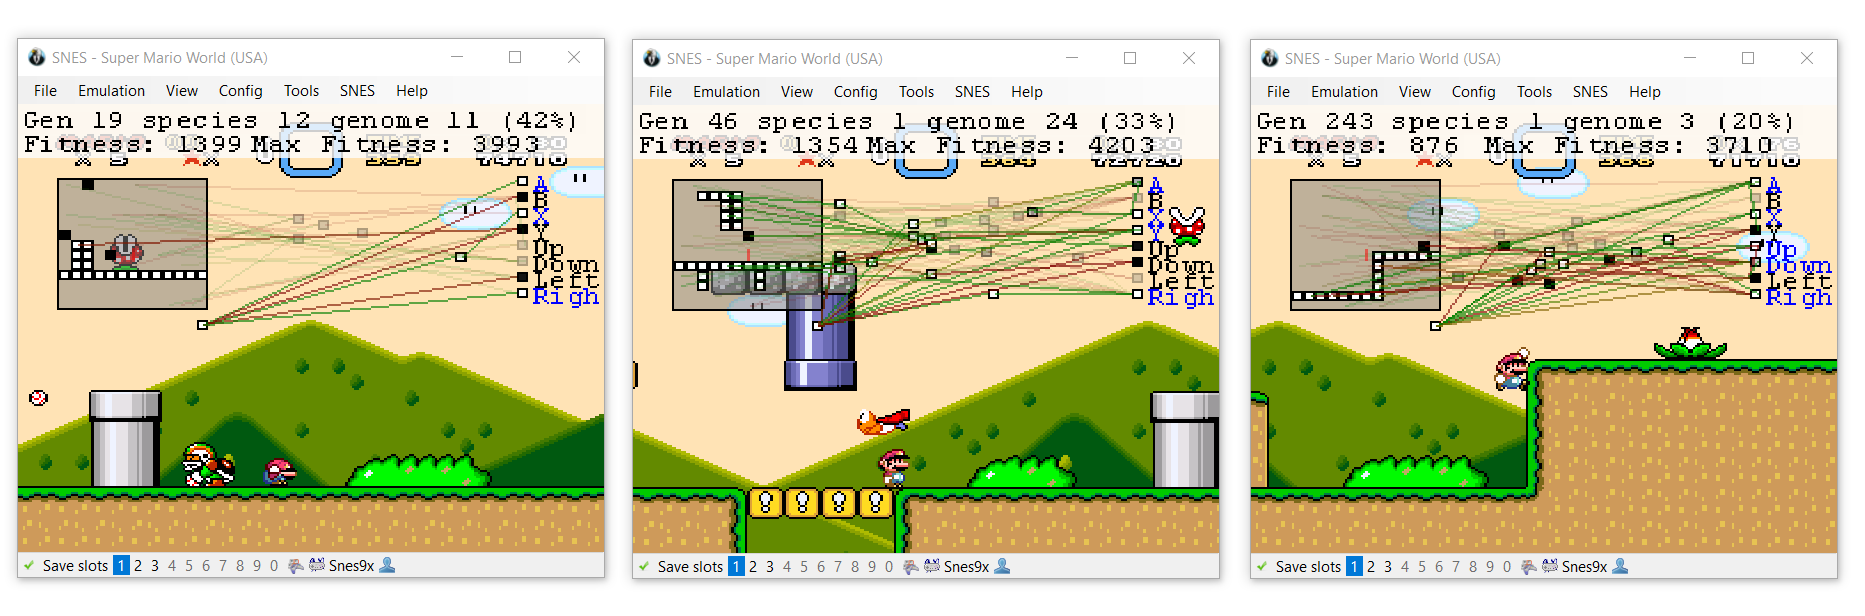
\includegraphics[width=1\textwidth]{graphics/mario/mario3}
			\caption{MarI/O simulation}
			\label{fig:mario}
		\end{figure}
		As mentioned in section \ref{sec:related:tools} MarI/O (see figure \ref{fig:mario}) is an implementation of \gls{neat}-algorithm written in \gls{lua}. It provides a solution for automatic learning of the game Super Mario World. In Super Mario World a level is a two dimensional map with steady as well as moving obstacles.
		Some of them block the path to the goal and others cause damage to Mario's health. A few of them give health upgrades to Mario or add coins to the players account, although the coins are ignored in the implementation of the \gls{ai}. Since there are many different positions in which Mario can stay and the speed of the game depends mostly of the player and his/her/its desicions the environment of Super Mario World is rather complex when compared to the second game Flappy Bird \ref{sec:analysis:flappy}.\\
		This complex world leaves the expectation that many hundred thousand runs are necessary to learn how to complete a level. However MarI/O implementation reached to goal after approximately $2664.29$ runs on average in the simulations described later in this section. Still 2 of the 9 simulations didn't reach the goal once.\\
		\todo{fitnessfunction, formlar? when was goal reached} \\
		Later in this section 3 figures with 3 homomorphic graphs will be shown. The three different figures display the success of the algorithm in different classes of initial population size. Since the \gls{neat}-algorithm used does not produce a deterministic amount of populations after the first generation (in general: Generation 0), the initial population size define these classes. There where three classes choosen with a scaling factor of 5 between them. These initial population sizes are 10, 50 and 250. Whether or not the initial population sizes are well chosen will be discussed shortly in the conclusion section (see \ref{sec:analysis:conclusion}) of this chapter. Depending on the evolution of the \gls{nn}, there are a certain amount of generations evolved. Every generation contains their own set of species. And on the other hand the species contain the genomes. In generation 0 every species contains only one genome each. The sum of all genomes in all species of a generation is called the population. In the cases where the initial population size is 10 or 50 over time to many generations where created to show a viewable graph in the end. That's why only 30 generations where picked in the display with even distances between them. Still a continuous line with the best run of a population is showed above all generations, even the skipped ones. \\
		In the later descriptions of the population classes there are two types of runs introduced. First is the "plot-run" which indicates the simulation and the graph. Inside of this graph there were many "runs" which represent the runs of the population (genomes) of each species. In figure \ref{fig:mario} there are 3 individual runs displayed. On average one plot-run consists of $4217.\overline{2}$ runs, whereas population 10 has $2828$ runs on average, population 50 contains of $4494.\overline{6}$ runs on average and population 250 of $5329$ runs averagely.\\
		In order to understand the fundamental differences of these simulations, the population classes are examined in more detail: 
		\paragraph{Population 10 / Generation 500}
			\label{par:mario10}
			\begin{figure}[h]
				\centering
				\begin{minipage}{0.33\textwidth}
					\centering
					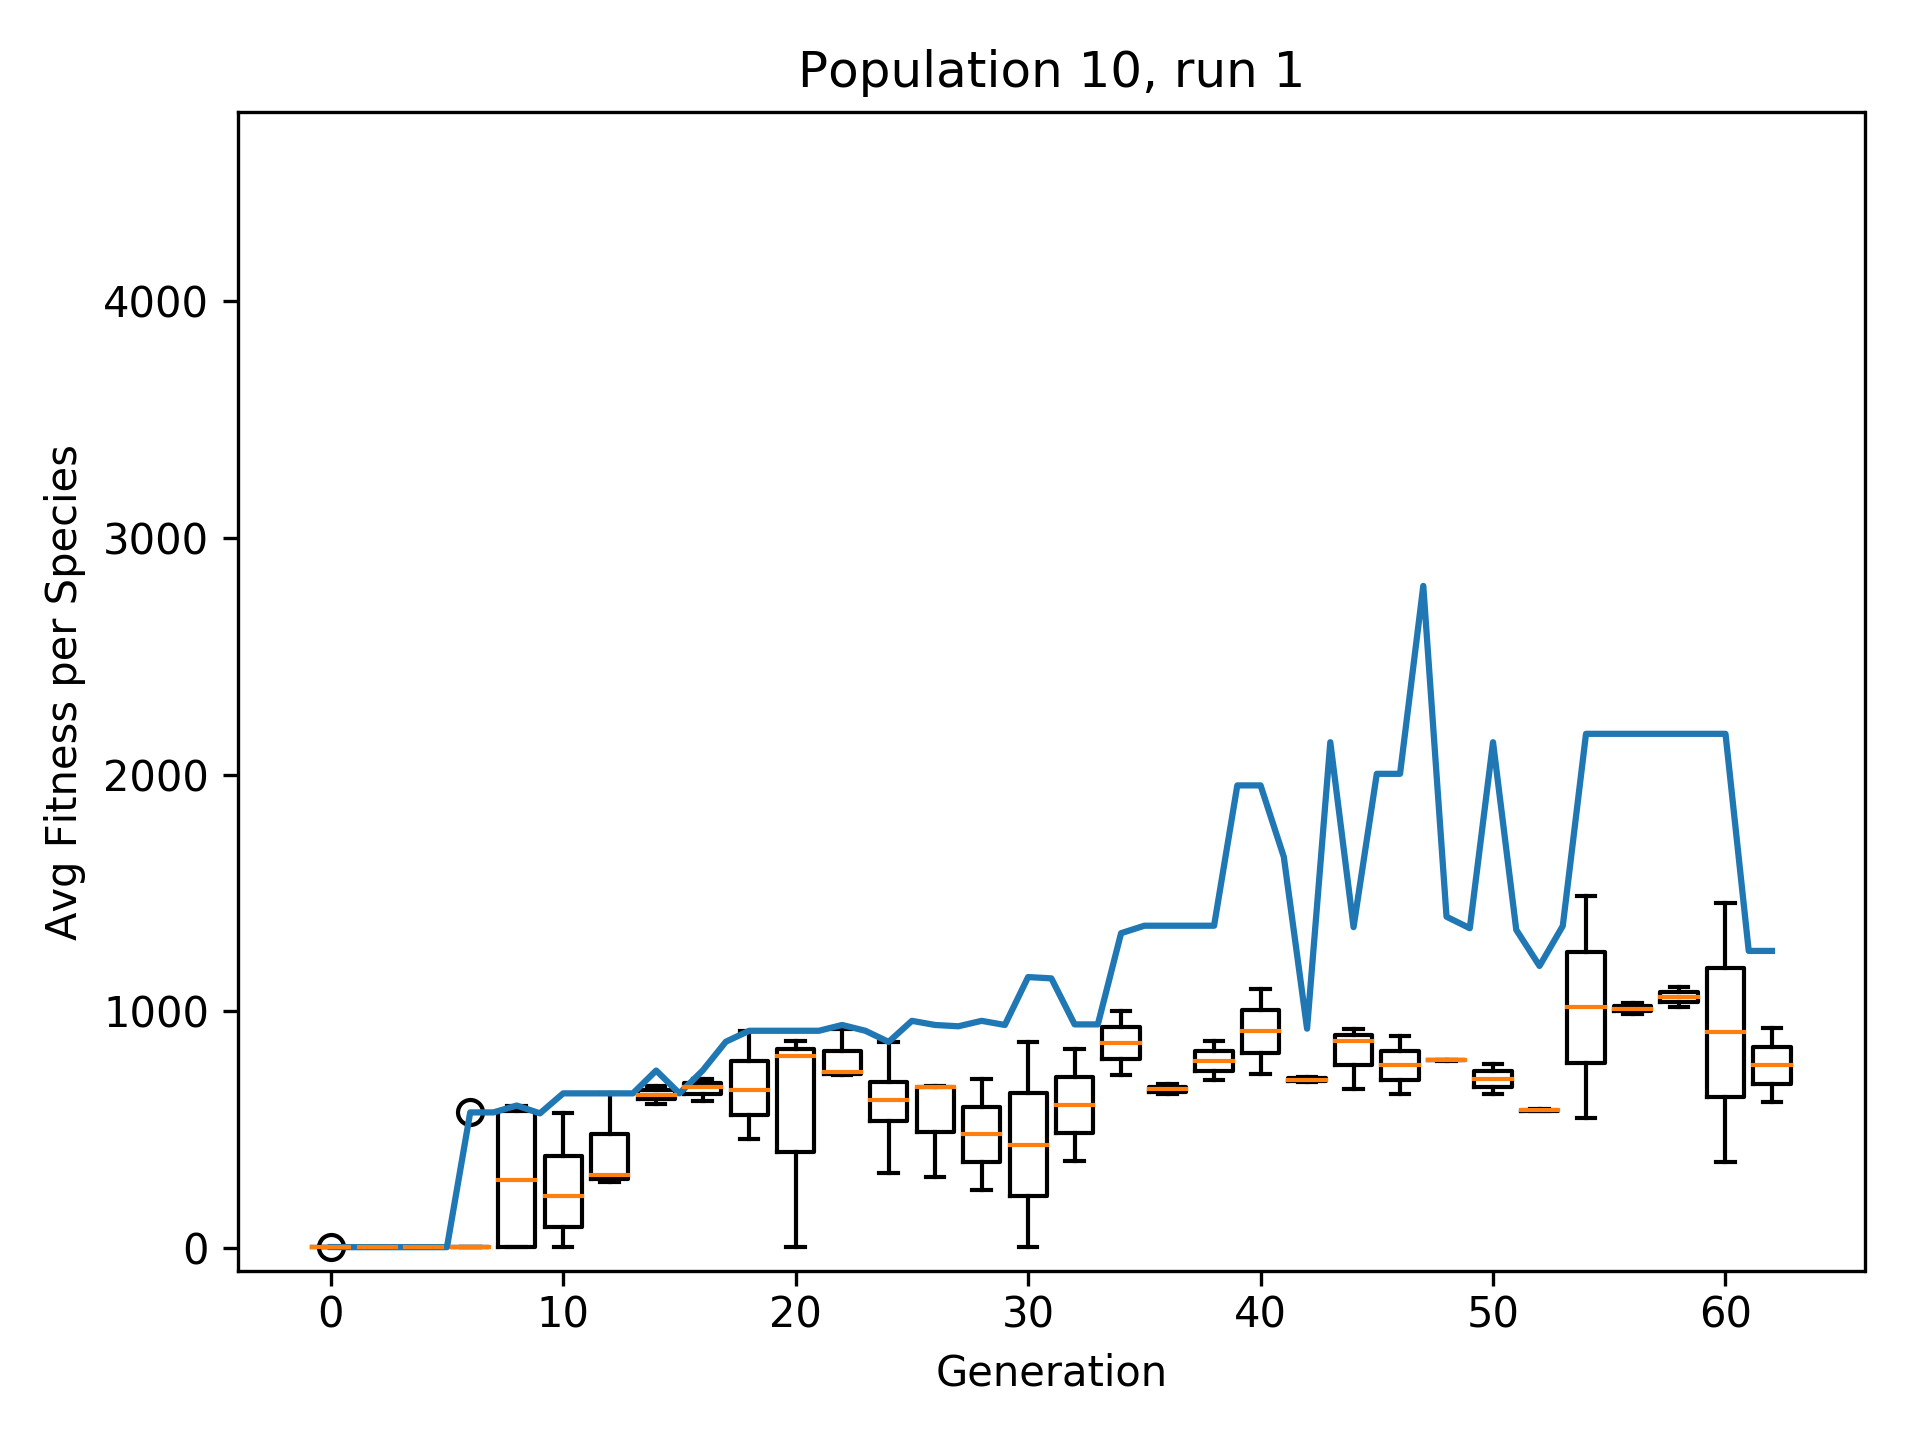
\includegraphics[width=1\textwidth]{graphics/mario/pop10_run1} % first figure itself
				\end{minipage}\hfill
				\begin{minipage}{0.33\textwidth}
					\centering
					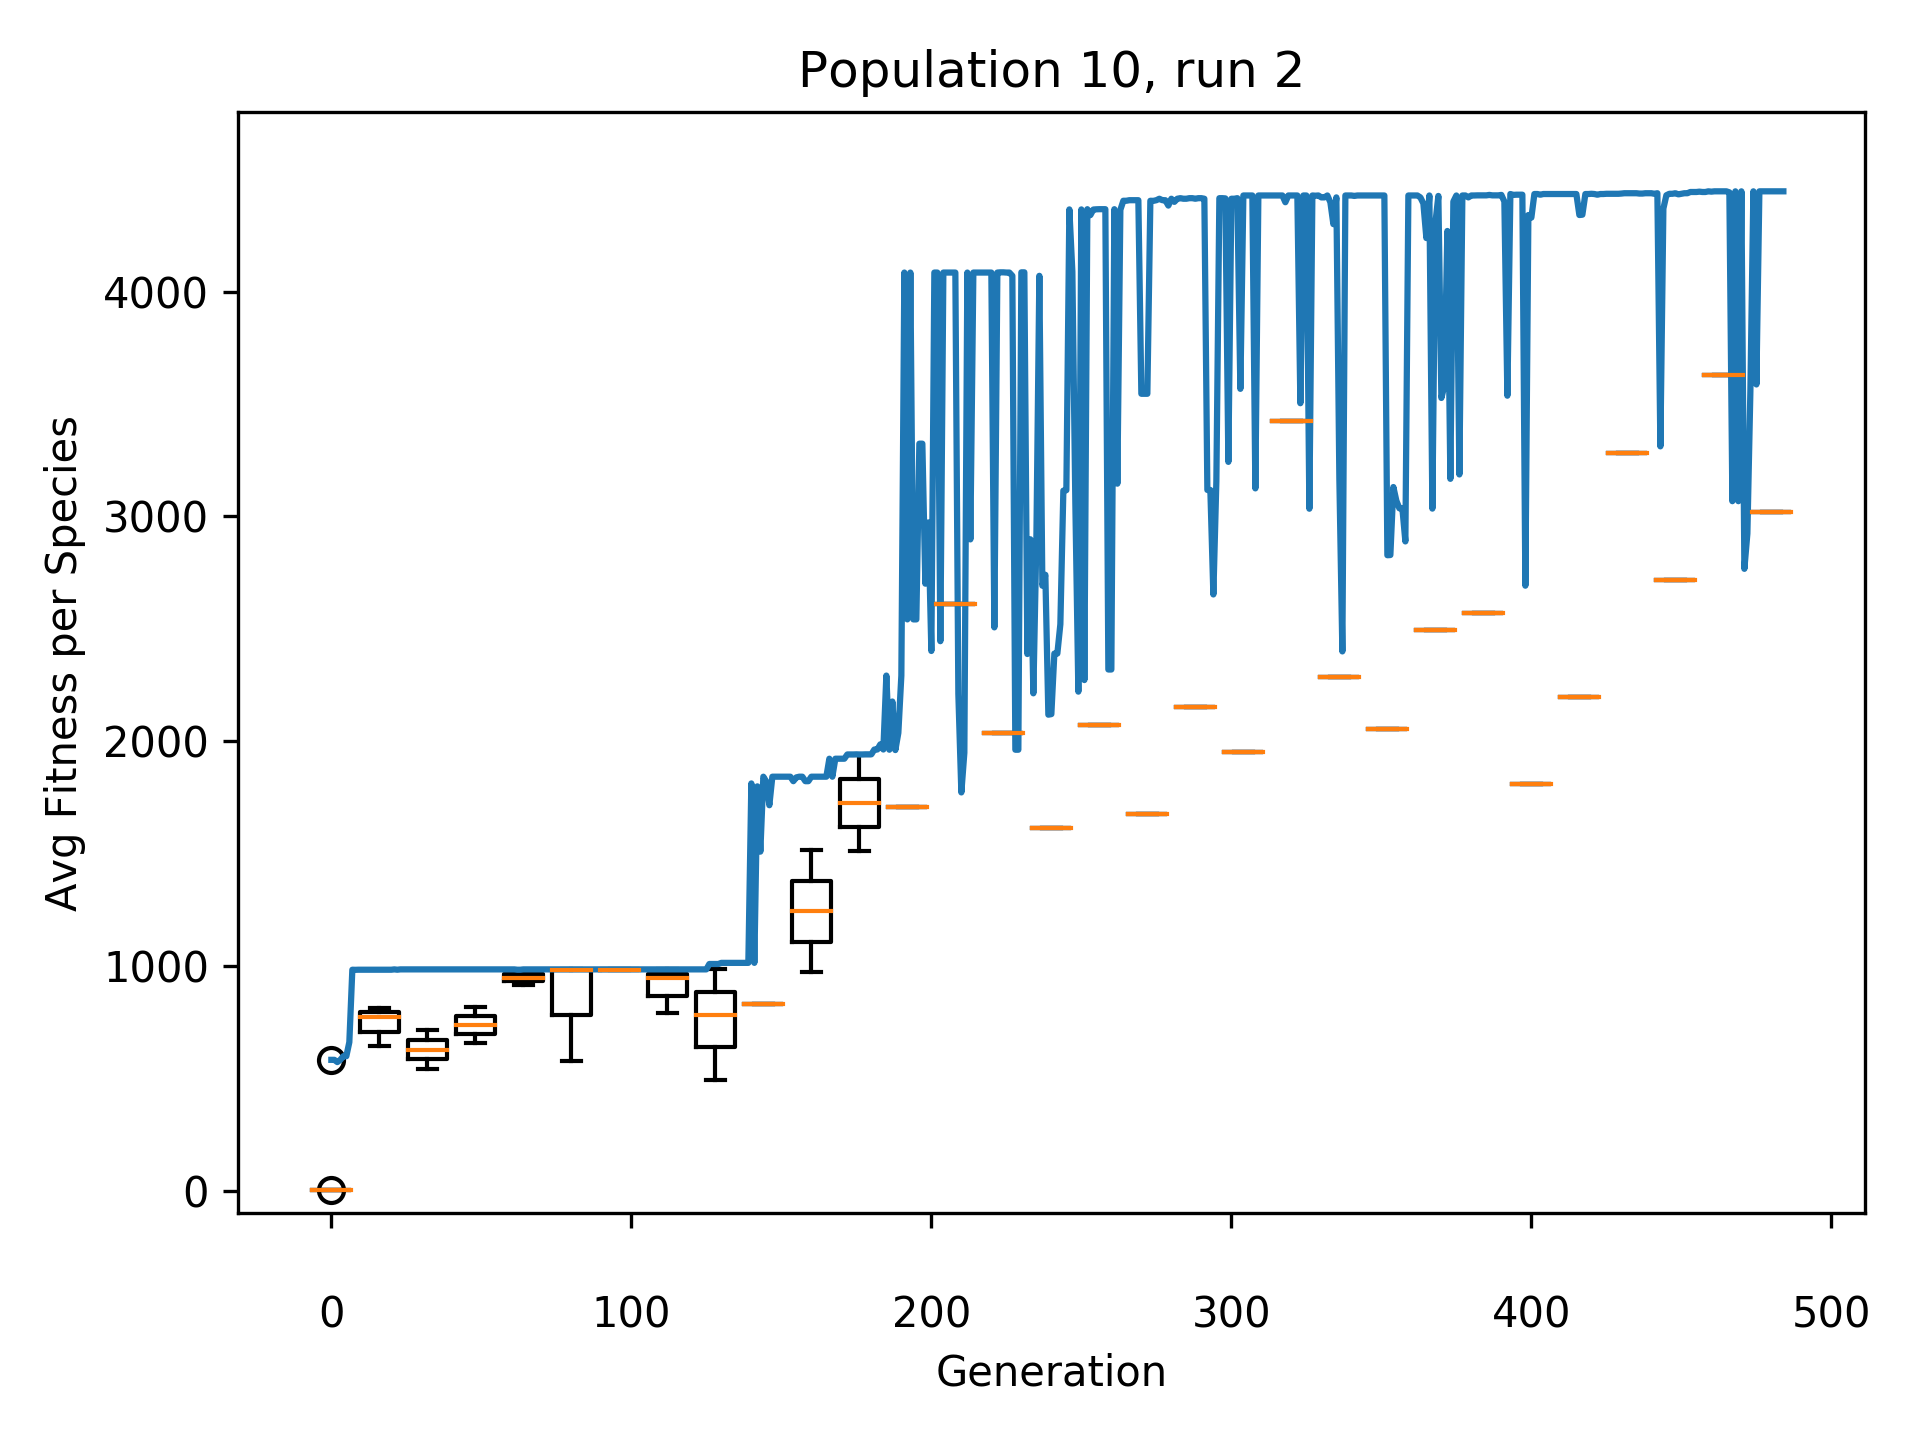
\includegraphics[width=1\textwidth]{graphics/mario/pop10_run2} % second figure itself
				\end{minipage}
				\begin{minipage}{0.33\textwidth}
					\centering
					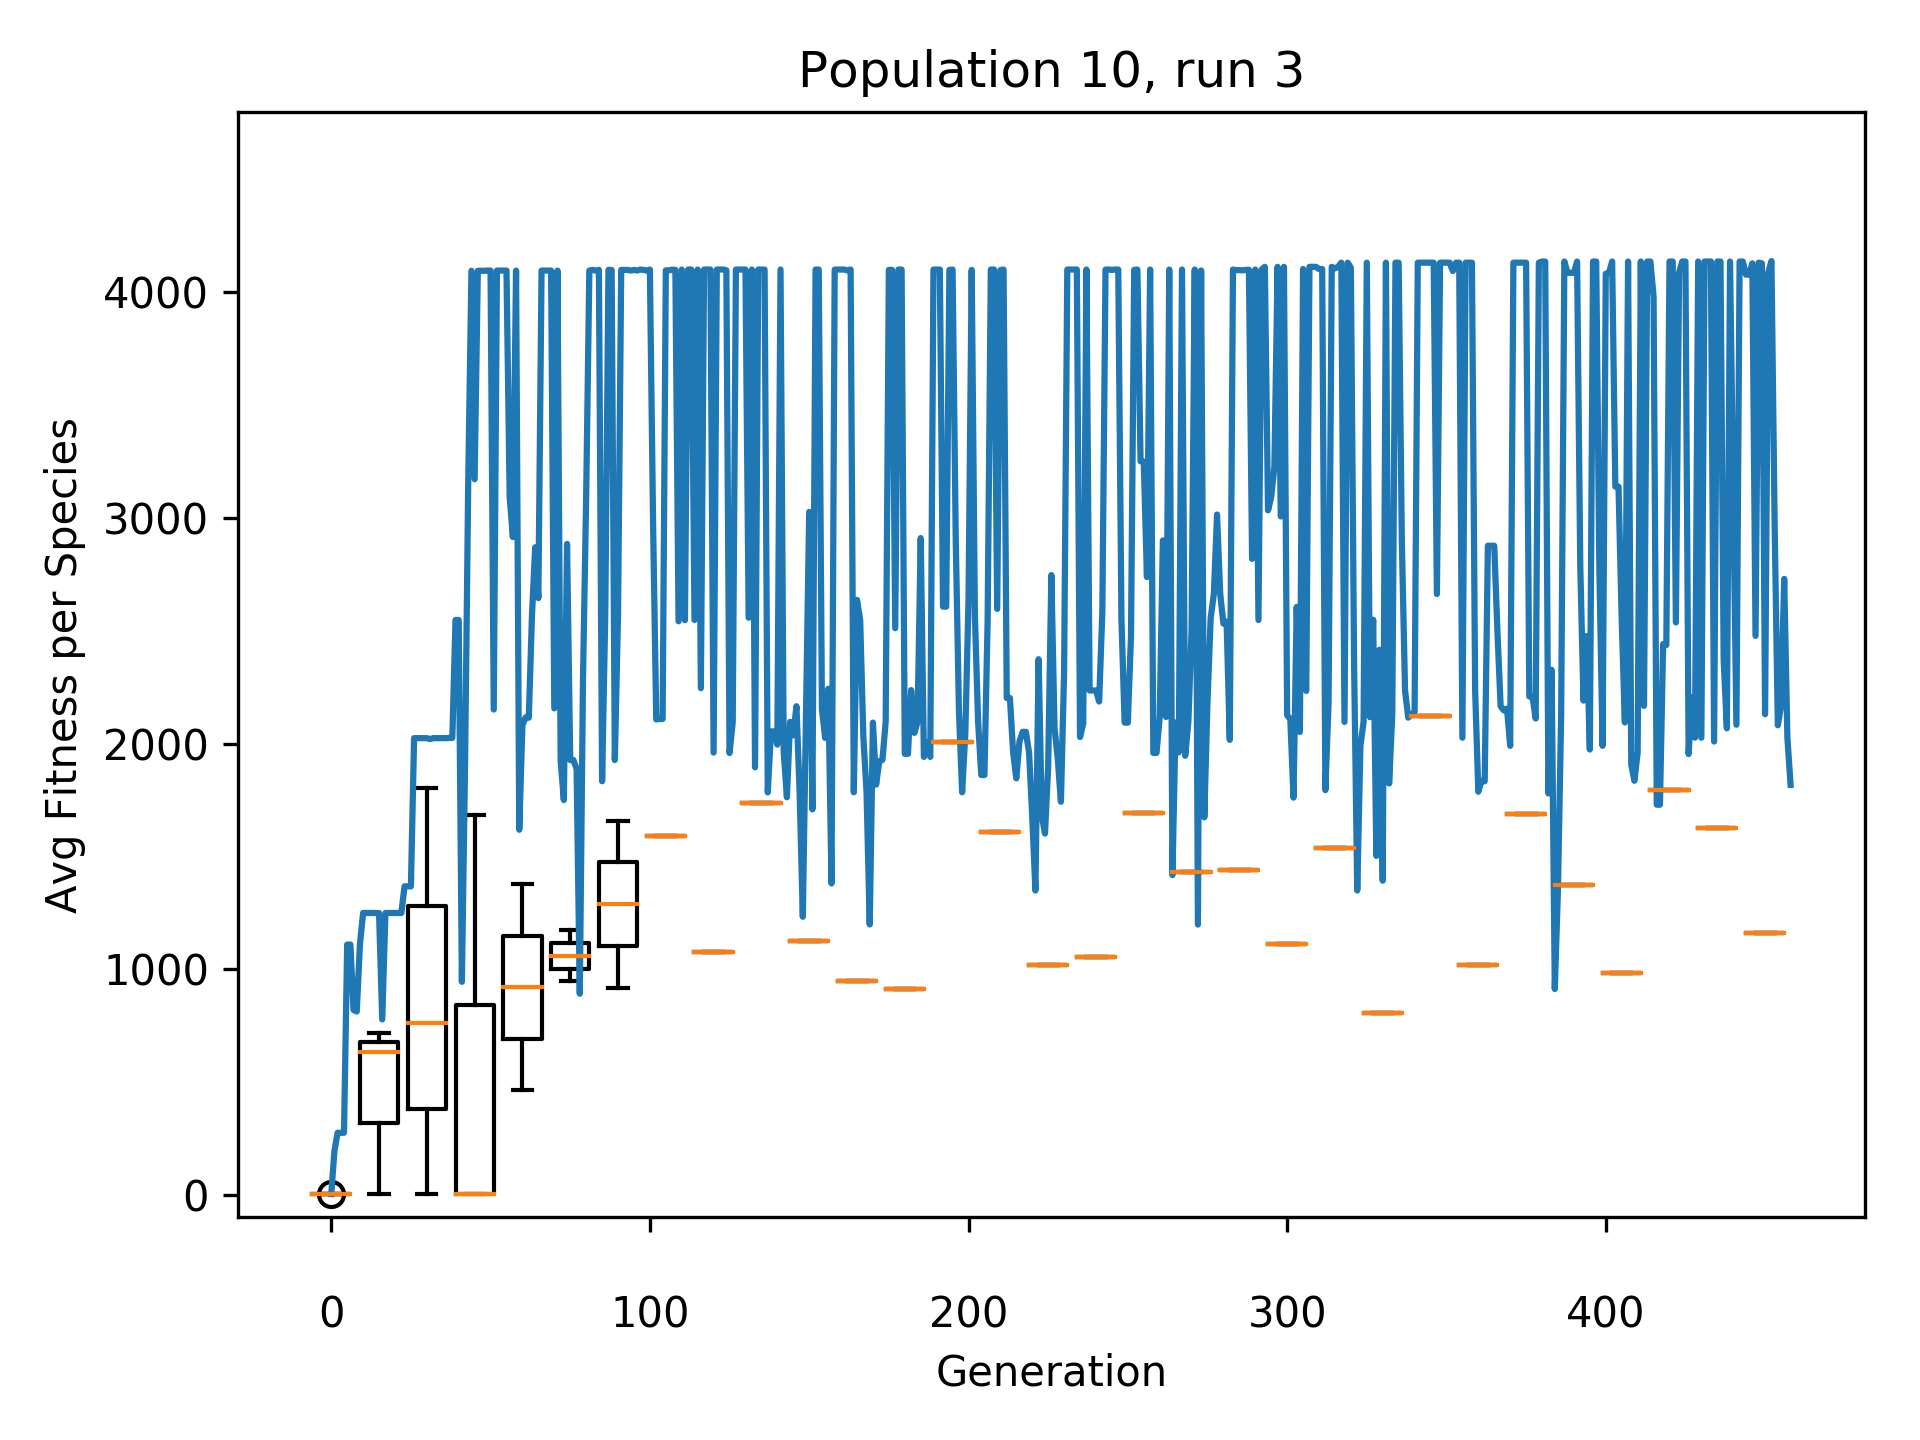
\includegraphics[width=1\textwidth]{graphics/mario/pop10_run3} % second figure itself
				\end{minipage}
				\caption{MarI/O Population 10}
				\label{fig:mario10}
			\end{figure}
			As it is visible in figure \ref{fig:mario10} the vertical axis shows the fitness score average of the genomes within a species. The horizontal axis portrays the generations containing the species. Each generation contains up to 10 populations which is divided into species and genomes within species. This species devision was made based on the \gls{neat} algorithm described in section \ref{sec:related:neat}. The best run of the genomes grouped by each generation is marked with a blue line. Therefore the blue line indicates the best overall run within a generation. Since the boxplot portrays the species's avarage score of each generation and the the blue line shows the best run per genome (population), the boxplot and the blue line rarely meet. Still the average population score is closer to the best run than in the next two population variants (see later in this section population 50 \ref{par:mario50} and population 250 \ref{par:mario250}). This can be calculated by taking the median of the species fitnesses and substracting that number from the best run of the genomes:
			$average\_distance = \frac{\sum\nolimits_{g_i \in generations} max(g_i.genomes) - median(g_i.species)}{|generations|}\approx1107$ whereas $g_i.genomes$ and $g_i.species$ are lists of the respective fitnesses. \\
			In the three plot-runs on average $334.\overline{6}$ generations were created, which results in a skipping of generations inside the graphics of around $11.1\overline{5}$ generations averagely, between two displayed generations. Unfortunately the first run crashed after generation 60. Still, because of the long runtime of the simulation the plot-run was kept. However, indicated by plot-run 2 and 3, the population growth started after this generation. As it can be seen in the 3rd plot-run of the figure \ref{fig:mario10}, sometimes runs over 3000 fitness score could be achieved even after the 30th generation. In plot-run 2 the average fitness of the single species left tend to rise, however more and longer plot-runs would be needed to test this hypothesis.\\
			In each generations there are up to 10 populations. \todo{(up to because of neat implementation check neat implementation}
			In the first generation (Gen 0) no mating was done. So in the first generation there where 10 species spawned with one genome each. In the 10th Generation on average only $4.\overline{3}$ species where left. After generation 50 maximum 3 species where left in all runs and after generation 190 in plot-run 2 and after generation 91 in plot-run 3, respectively, only 1 species was left for mating. The mating results into the corssover of species.\\
			All runs except plot-run 1 reached the goal (the end of the level) multiple times which can be seen by the fitnesscore being over 4000. However plot run 3 reached the goal the earliest with runs over 4096 starting from generation 44. Still there was the most overall regress made in plot run 3. This can be calculated by adding the differences between the best runs of each generation if the difference was negative: $average\_regress = \frac{\sum\nolimits_{g_i \in generations} min(max(g_i.genomes) - max(g_{i-1}.genomes), 0)}{|generations|}\approx-348$ again whereas $g_i.genomes$ is a list of the fitnesses of each genome inside the generation. The regress of plot-run 1 was $-88.27$ approximately and of plot-run 2 was around $-109.98$.\\
			In plot-run 1 the $average\_fitness\_increase =  \frac{\sum\nolimits_{g_i \in generations} max(g_i.genomes) - max(g_{i-1}.genomes)}{|generations|}\approx19.87$ was the biggest of the three plot-runs since the first plot-run ended early and plot-run 3 had many drawbacks. The average fitness increase of plot-run 2 was around $7.97$ and of plot-run 3 was only $3.95$ approximately. Since it is only slightly possible to extend the maximum score above the score of 4000 and plot-run 1 has never reached this ranking, plot-run 1 pointed out to have the best score increase per round. Every successful round, whereas Mario reached the goal will only minimize the fitness increase when averaged with the generation count. In another words, for an infinitely large amount of generations the $average\_fitness\_increase$ is expected to converge to $0$ since the game has and end-state in contrast to the game Flappy Bird, as it can be seen in section \ref{sec:analysis:flappy}. In mathematical terms: $\lim\limits_{n \to \infty} average\_fitness\_increase(n) = 0$, whereas the $average\_fitness\_increase(n)$ is defined as the average fitness increase of a set of n generations.
		
		\paragraph{Population 50 / Generation 100}
			\label{par:mario50}
			\begin{figure}[h]
				\centering
				\begin{minipage}{0.33\textwidth}
					\centering
					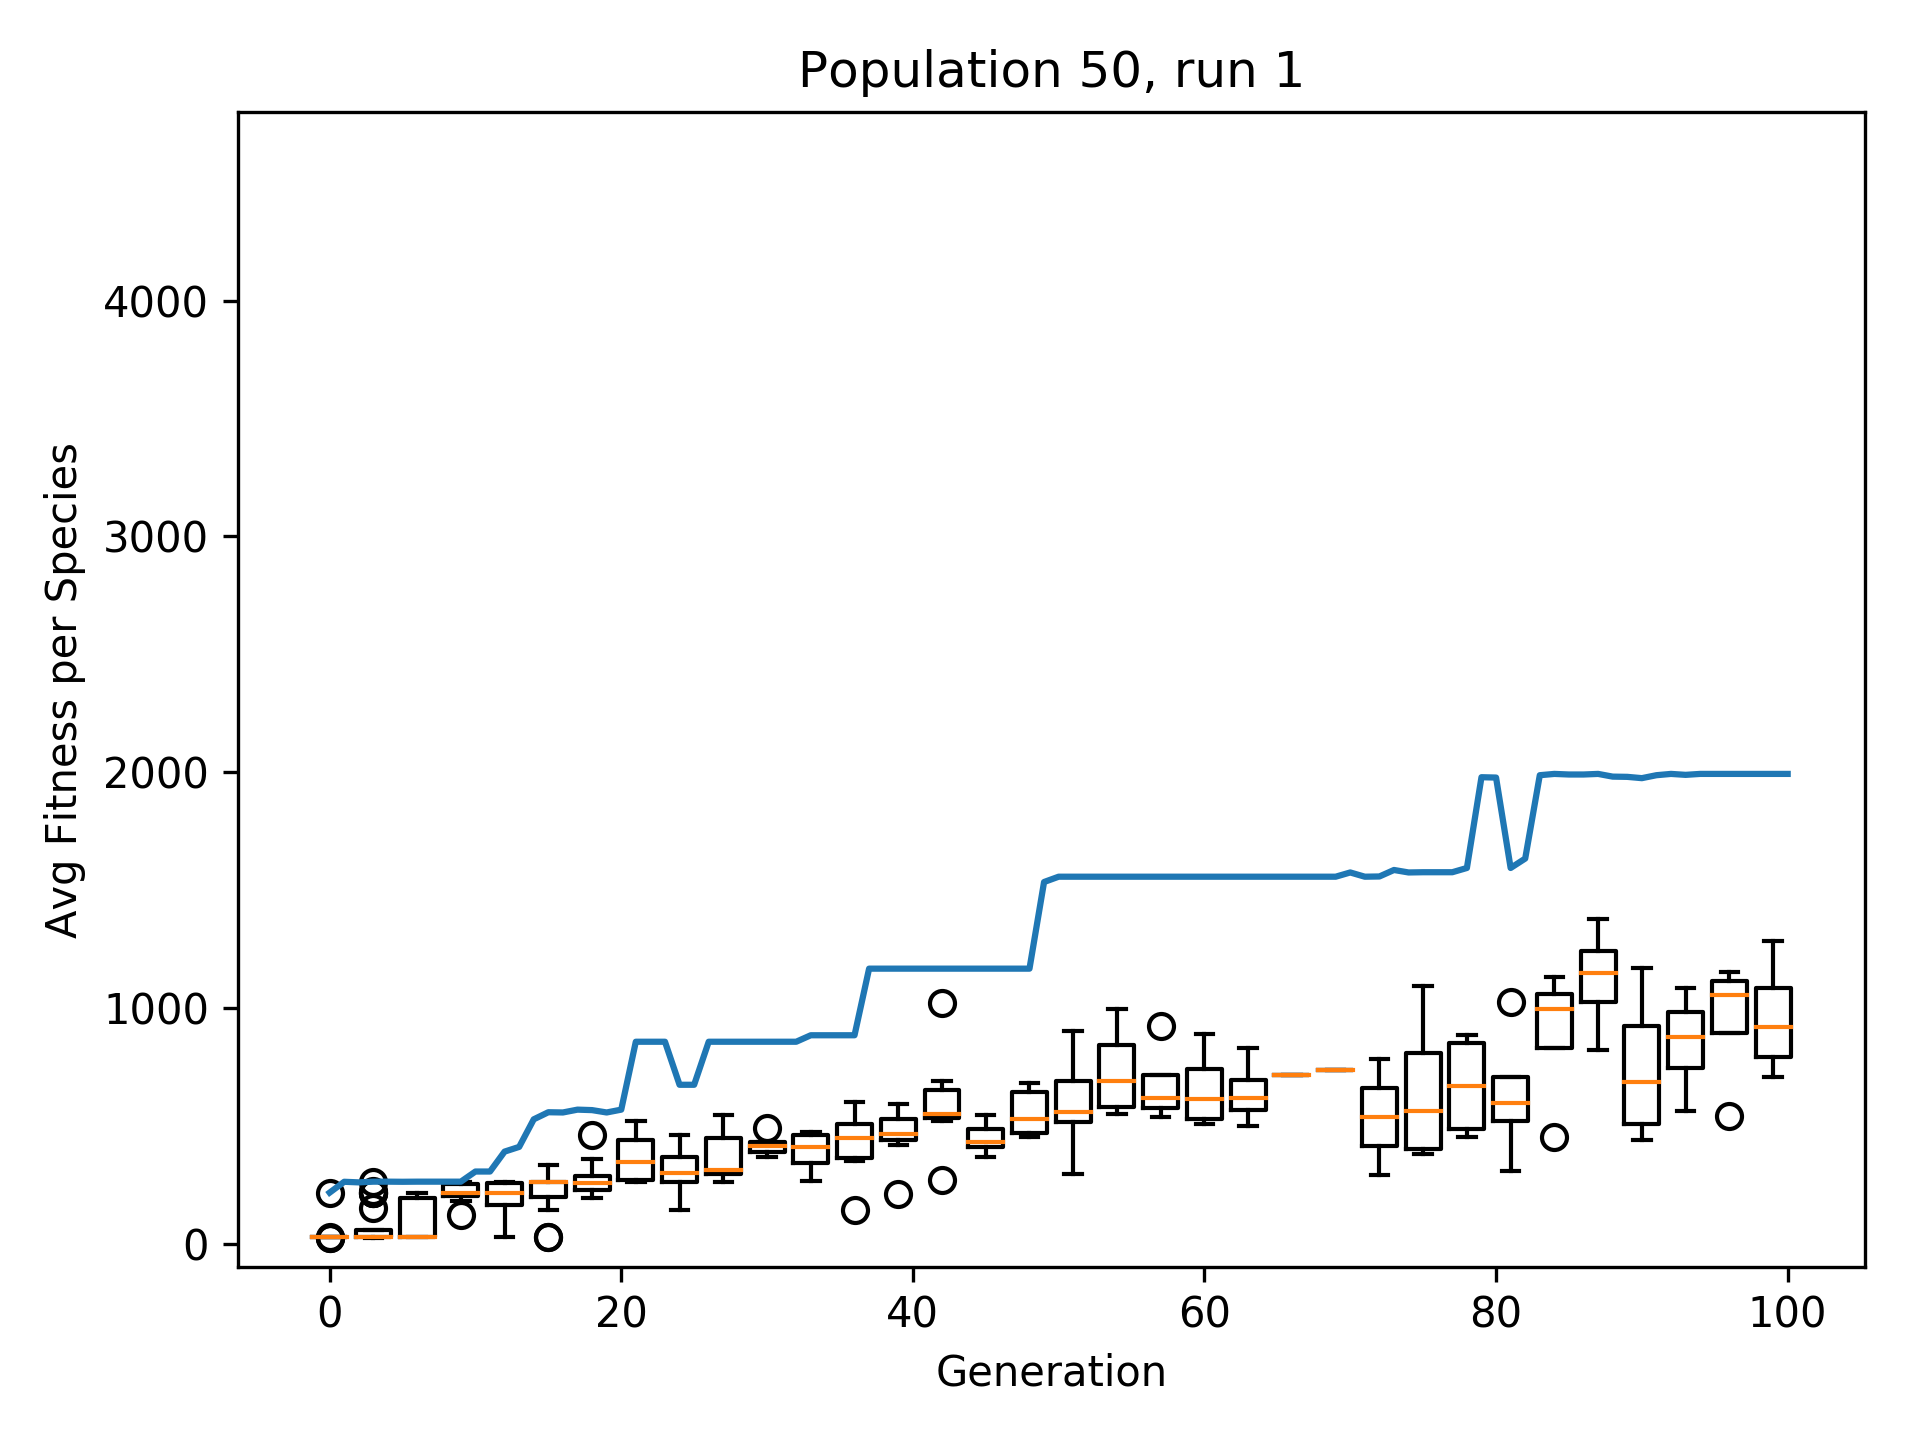
\includegraphics[width=1\textwidth]{graphics/mario/pop50_run1} % first figure itself
				\end{minipage}\hfill
				\begin{minipage}{0.33\textwidth}
					\centering
					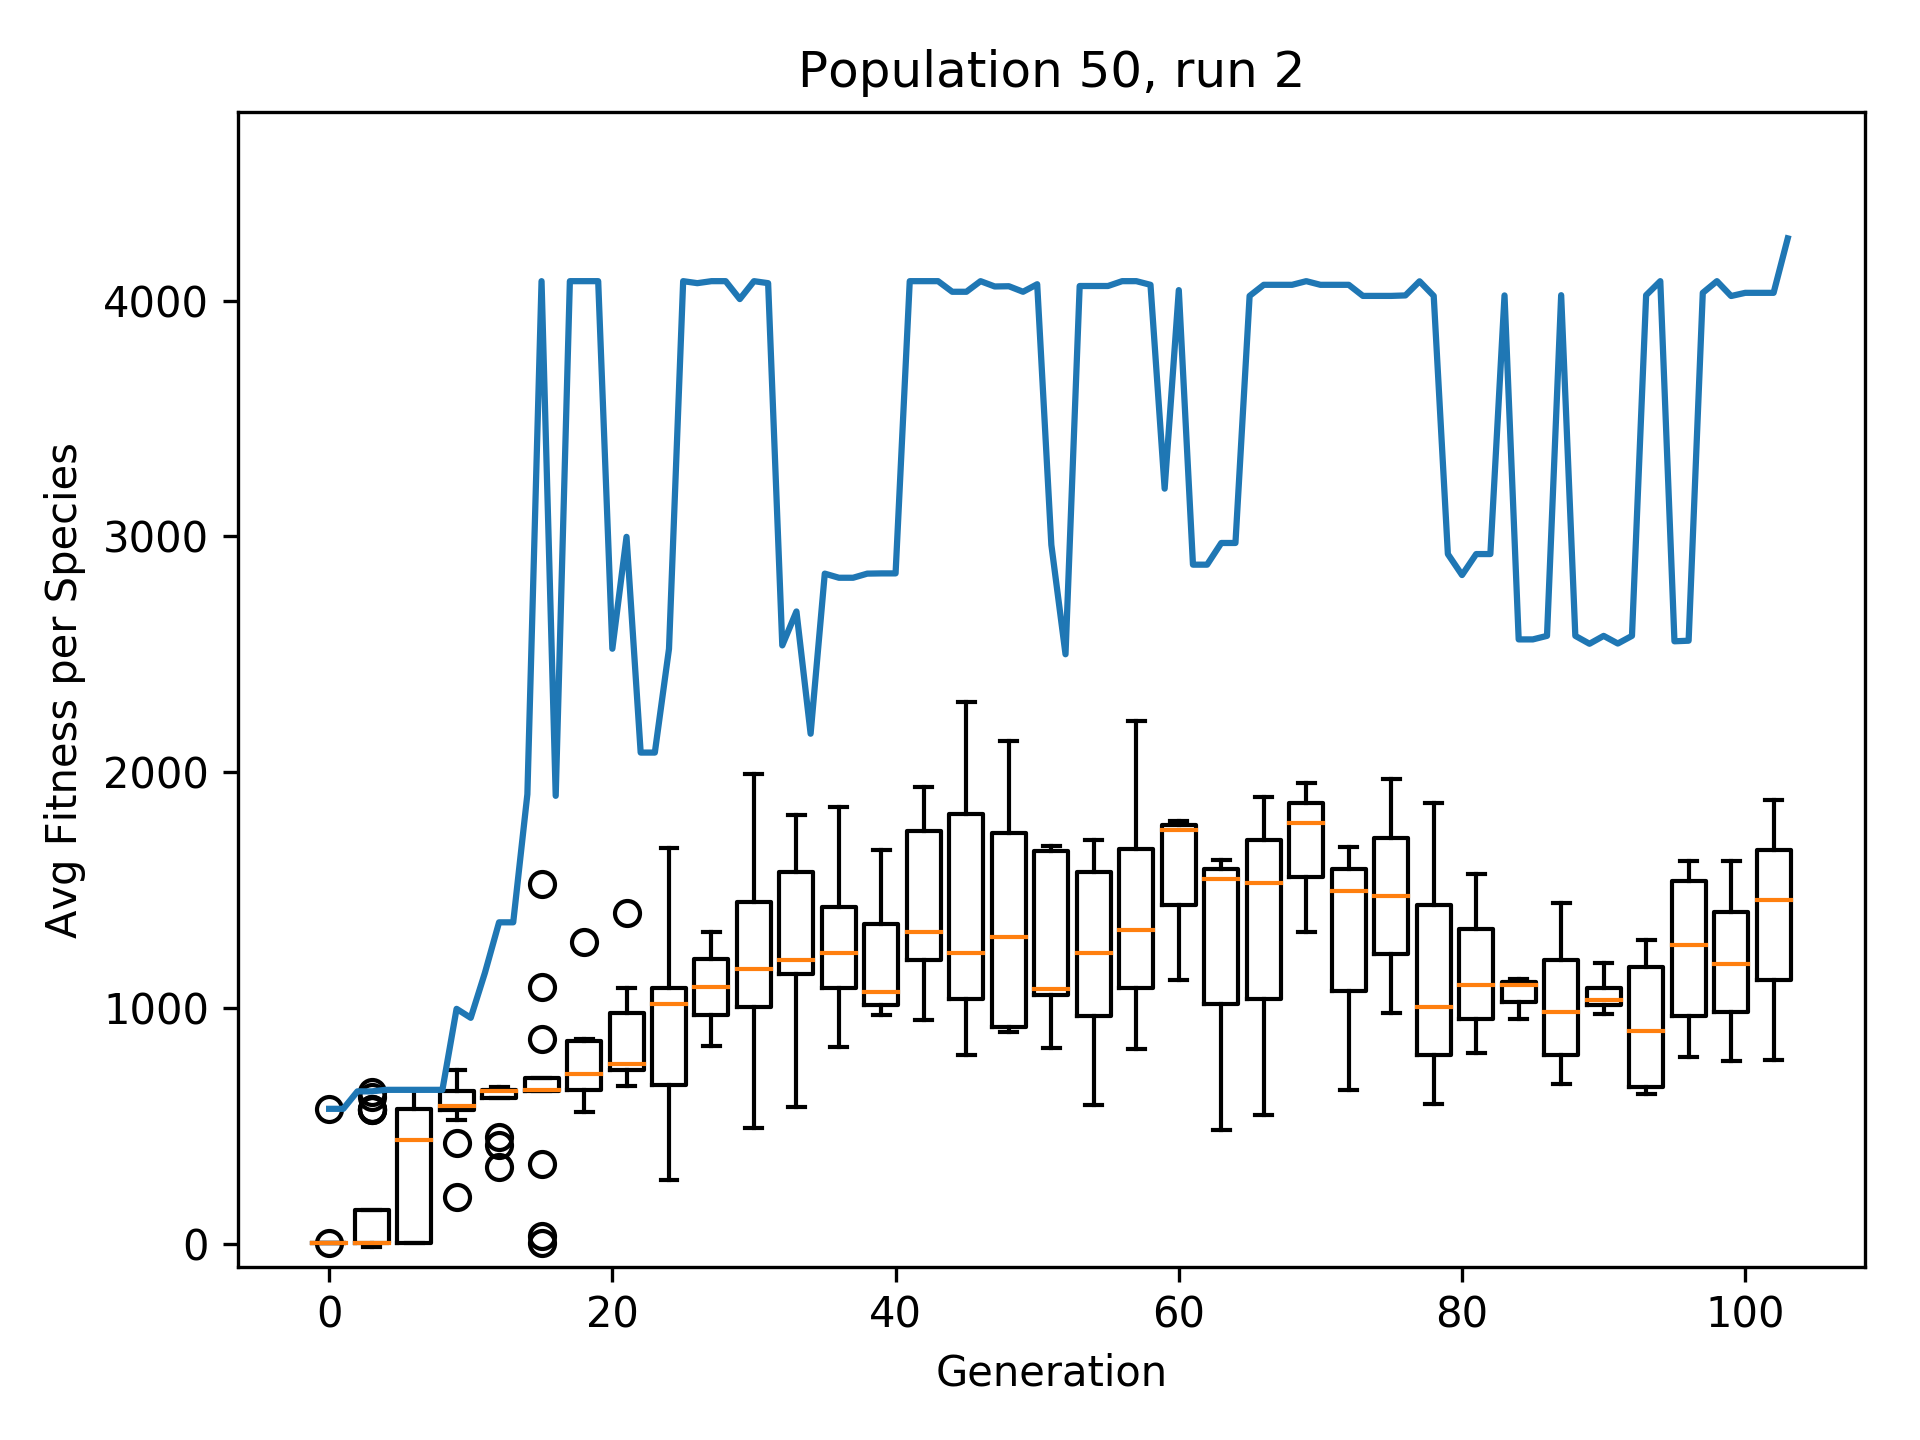
\includegraphics[width=1\textwidth]{graphics/mario/pop50_run2} % second figure itself
				\end{minipage}
				\begin{minipage}{0.33\textwidth}
					\centering
					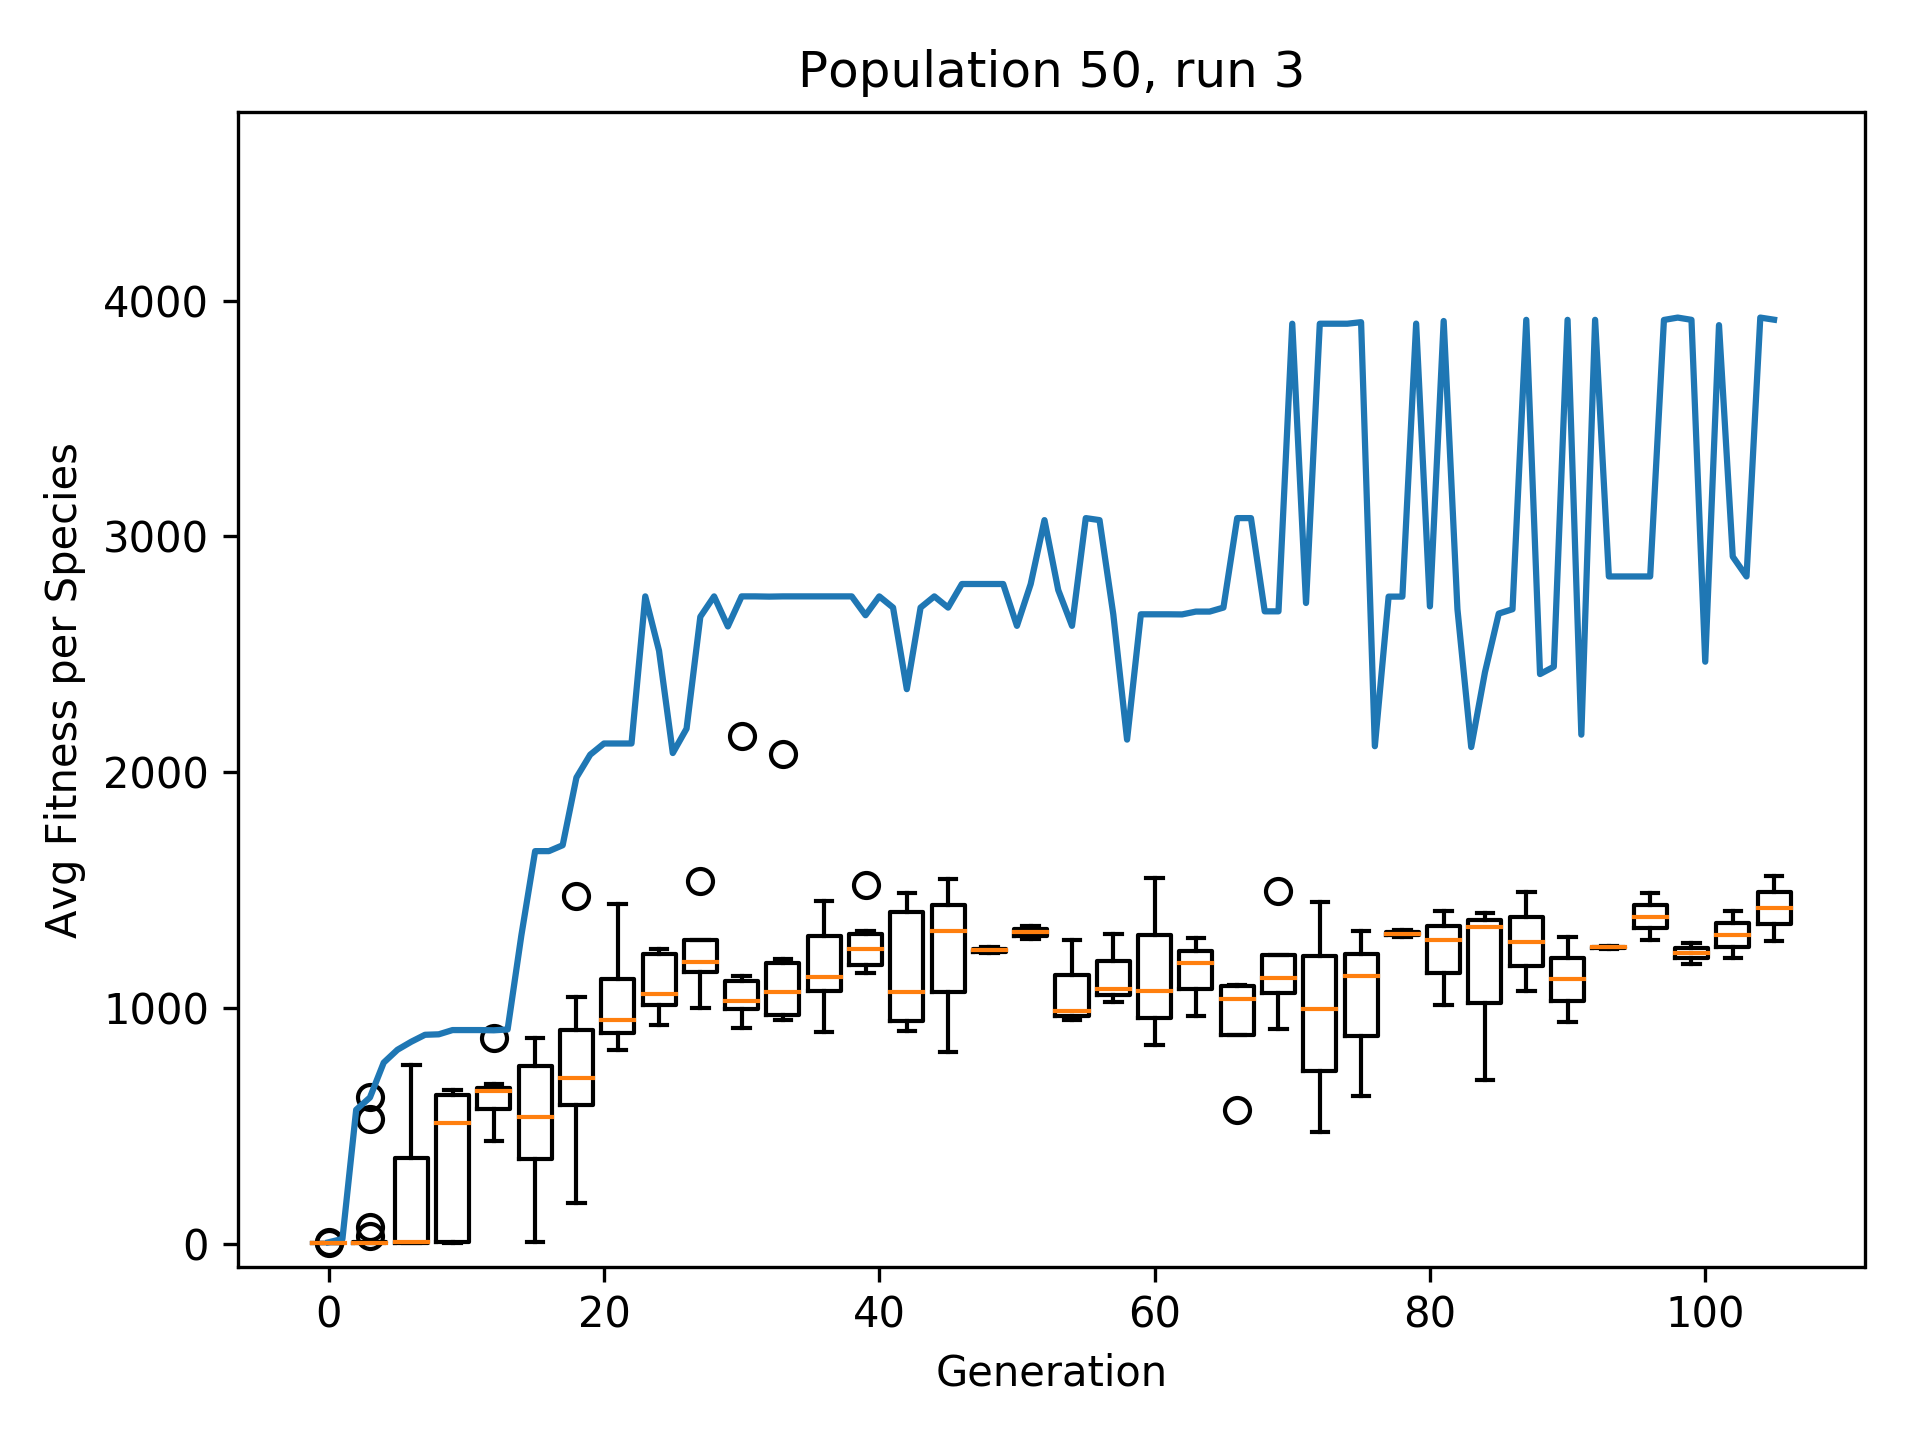
\includegraphics[width=1\textwidth]{graphics/mario/pop50_run3} % second figure itself
				\end{minipage}
				\caption{MarI/O Population 50}
				\label{fig:mario50}
			\end{figure}
			In this setup the population count is up to 50, again distributed into species and genomes within species according to the MarI/O NEAT implementation. The $average\_distance$  between the median of the species of each generation to the best genome run of this generation is bigger than that of the simulation with it's initial population size of 10 but it is smaller than in the last case. The $average\_distance$ was calculated as described in the previous simulation (population 10 \ref{par:mario10}) and the value is approximately $1406$.\\
			In this simulations the plot-runs where executed until there where over 100 generations (101 generations in plot-run 1, 104 in plot-run 2 and 106 in plot-run 3). This results in an average skipping of 3.456 generations between the display of two generations.\\
			In generation 0 there where 50 species spawned, again, with one genome each. In the 10th generation there where 15 species left on average. At the end of generation 100 on average $3.\overline{3}$ species where left from the initial 50 generations.\\
			Interestingly the plot-run 1 couldn't learn to reach the goal. From this data it is not trivial to predict if the breakthrough would have started within the next 50 generations or if this plot-run would have stayed low in it's fitness score, since there are no clear patterns to find in the graphical representation of these runs. In order to answer on this question more profoundly, further and longer plot-runs have to be made and the big jumps between the fitness scores of each neighbour generation would have to be analysed.\\
			Plot-run 2 and 3 had more luck in reaching the end, however plot-run 3 had more stability in it's high score results between generations. Still after generation 70 plot-run 3 also shows stronger differences between it's generation's heigh scores. Nevertheless, plot-run 2 reached the goal the earliest. The first time plot-run 2 achieved a fitness-score over 4000 was in generation 15 (it reached a score of $4082.5$), whereas plot-run 3 reached a maximum score of $3928$ in generation 98. Still plot-un 3 reached to goal with a score of $3902$ the first time in generation 70. The 3rd plot-run has the highest $average\_fitness\_increase\approx36.92$ of the three plot-runs. Plot-run 1 has an $average\_fitness\_increase$ of $17.58$ approximately and plot-run 2 of $35.5$ precisely.\\
			Plot-run 2 and 3 have similar $average\_regress$ values with approximately $-158.02$ for plot-run 2 and $-152.37$ for plot-run 3. Because of the early end of general low performance of plot-run 1 the $average\_regress$ is also the lowest with $-6.30$. Still there where only 15 cases where the succeeding generation performed worse than the previews in plot-run 1 whereas there where 29 of these cases in plot-run 2 and 30 in plot-run 3. This indicated a certain stability in the first plot-run although the maximum score remained far lower than $3000$.
		
		
		\paragraph{Population 250 / Generation 30}
			\label{par:mario250}
			\begin{figure}[h]
				\centering
				\begin{minipage}{0.33\textwidth}
					\centering
					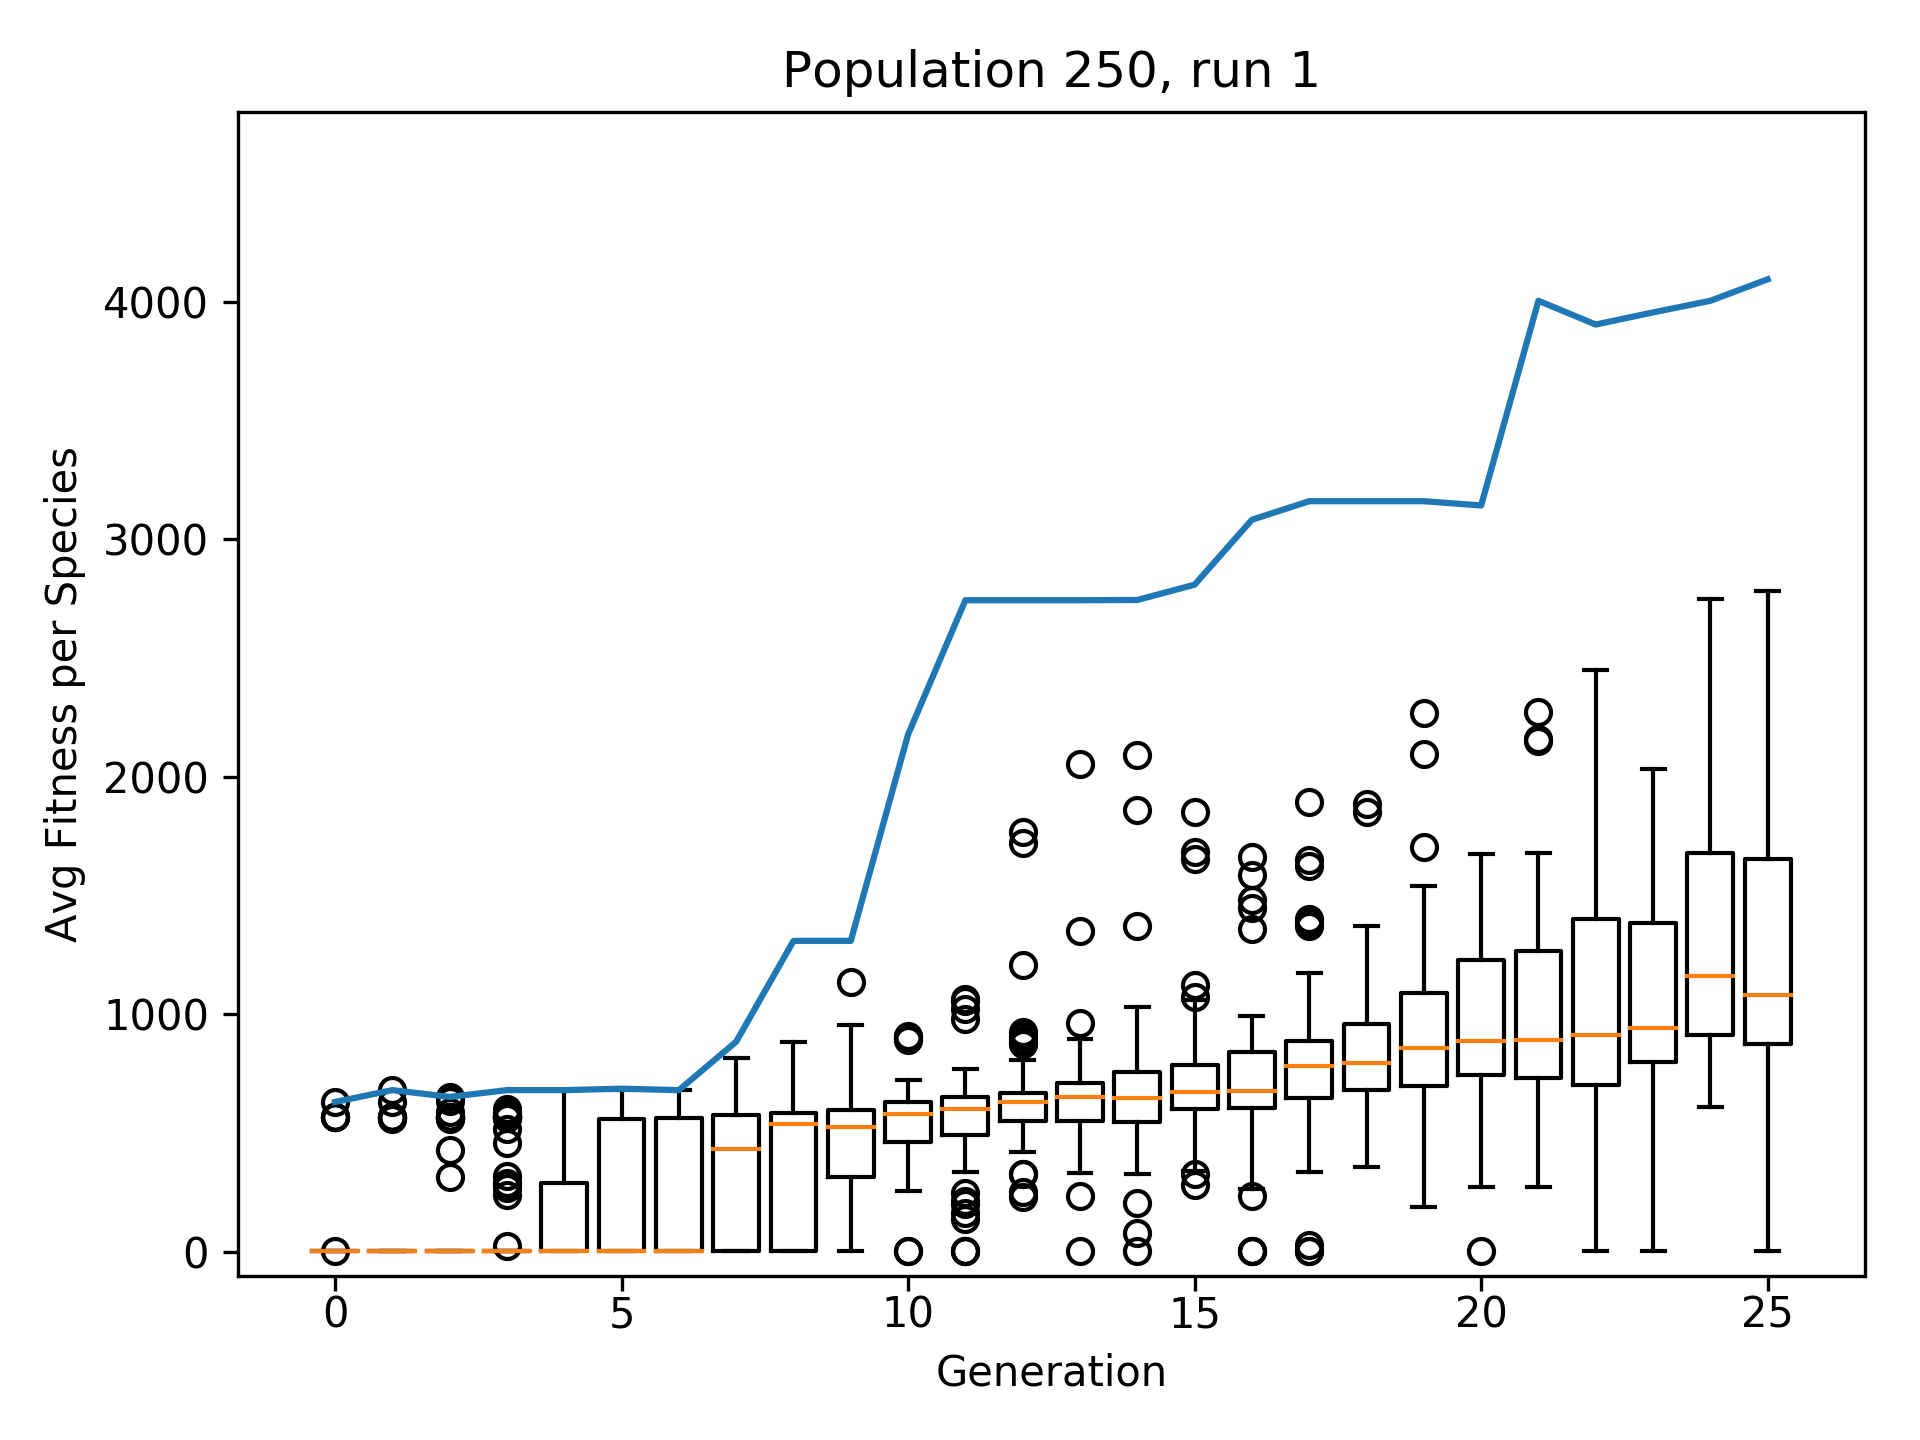
\includegraphics[width=1\textwidth]{graphics/mario/pop250_run1} % first figure itself
				\end{minipage}\hfill
				\begin{minipage}{0.33\textwidth}
					\centering
					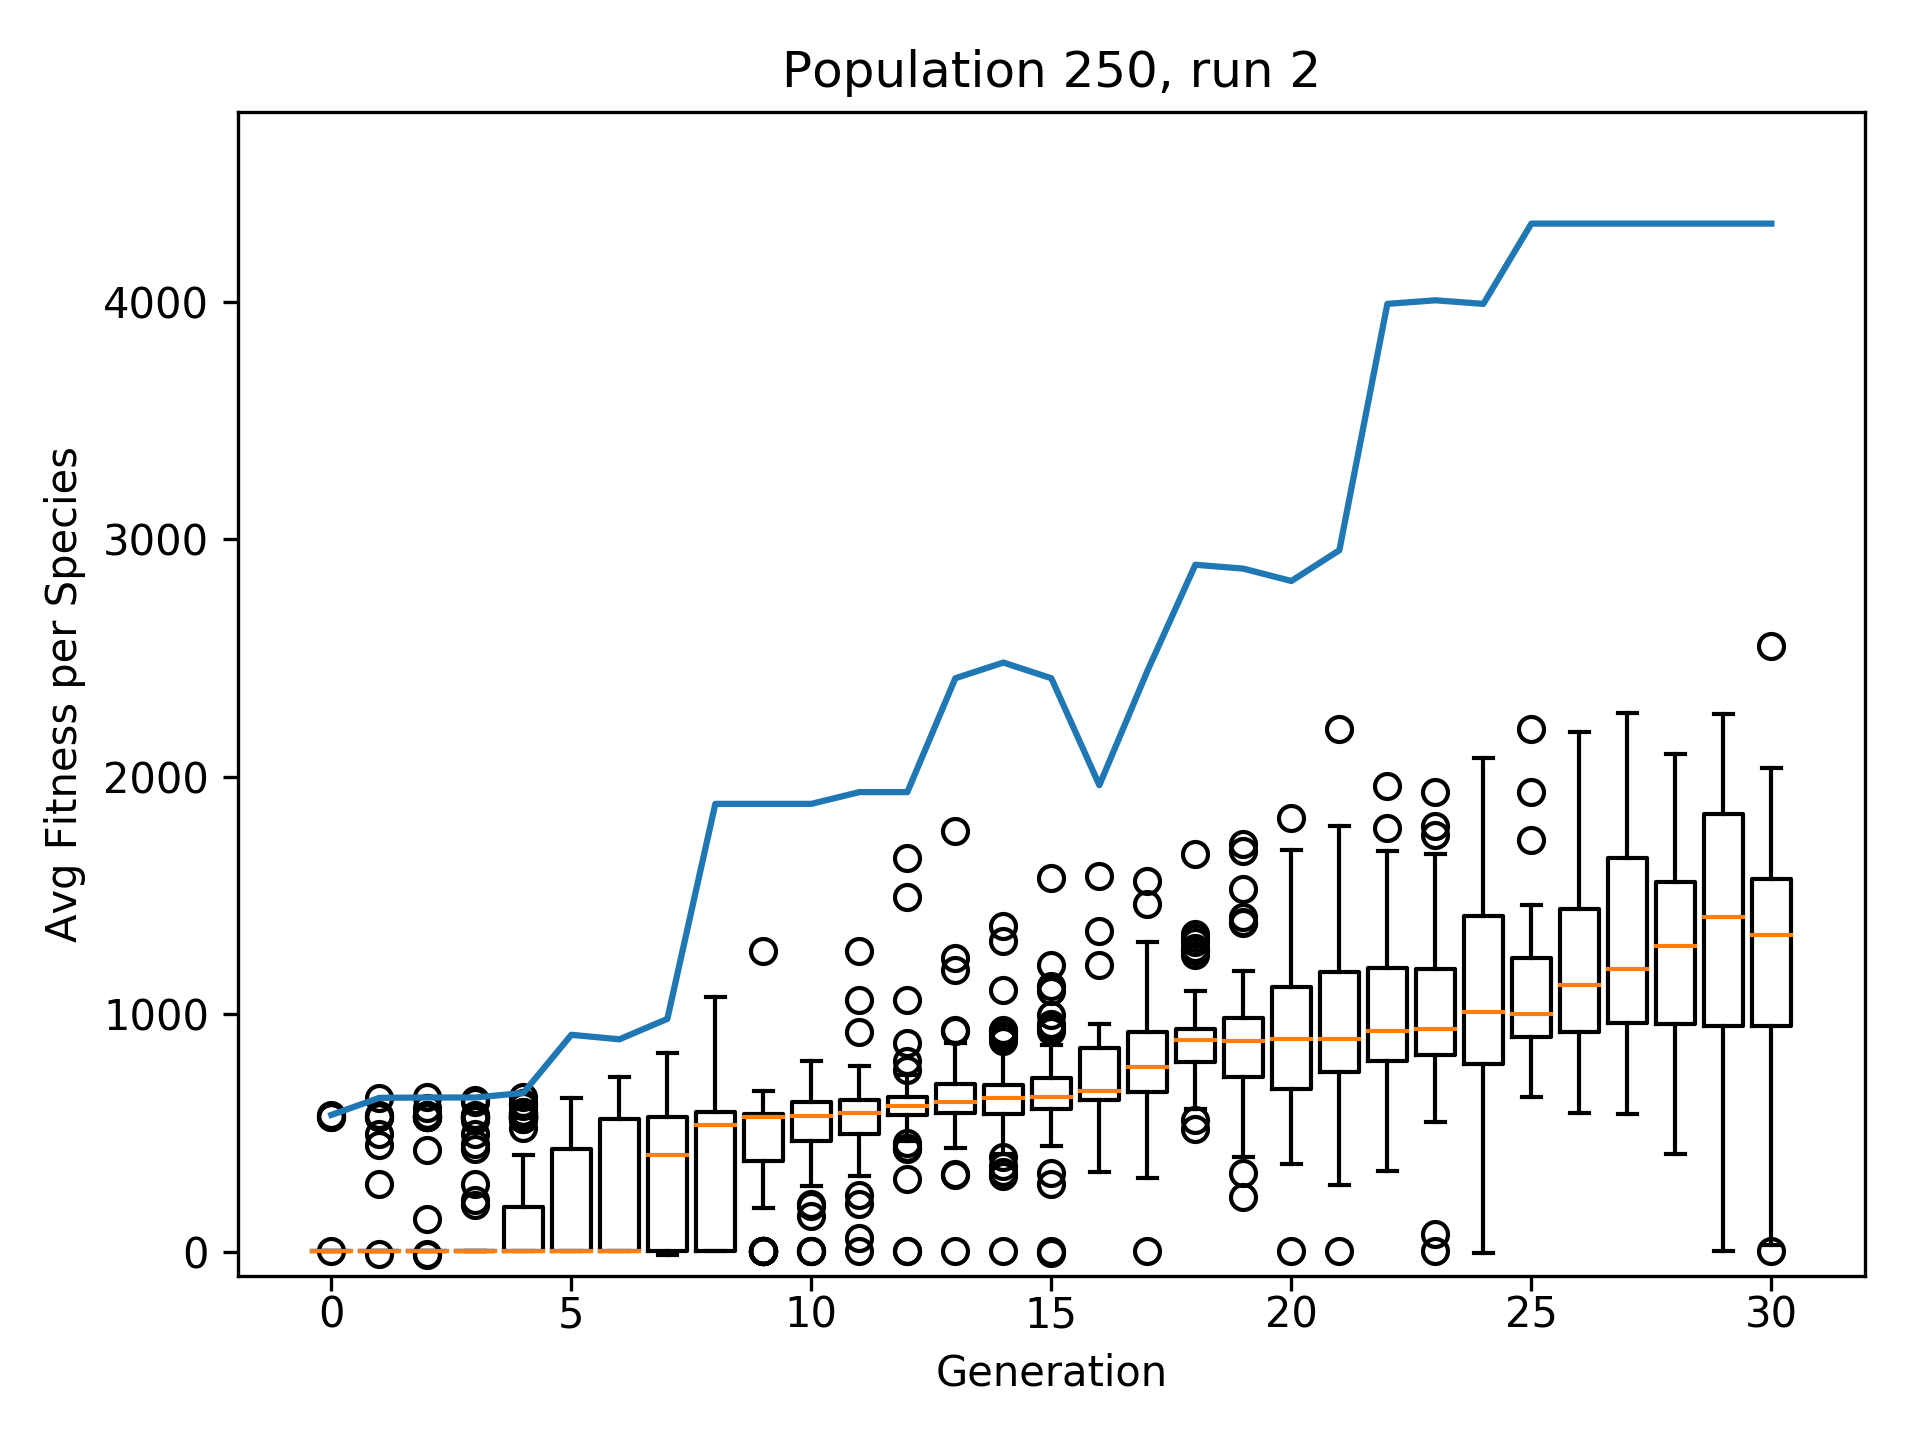
\includegraphics[width=1\textwidth]{graphics/mario/pop250_run2} % second figure itself
				\end{minipage}
				\begin{minipage}{0.33\textwidth}
					\centering
					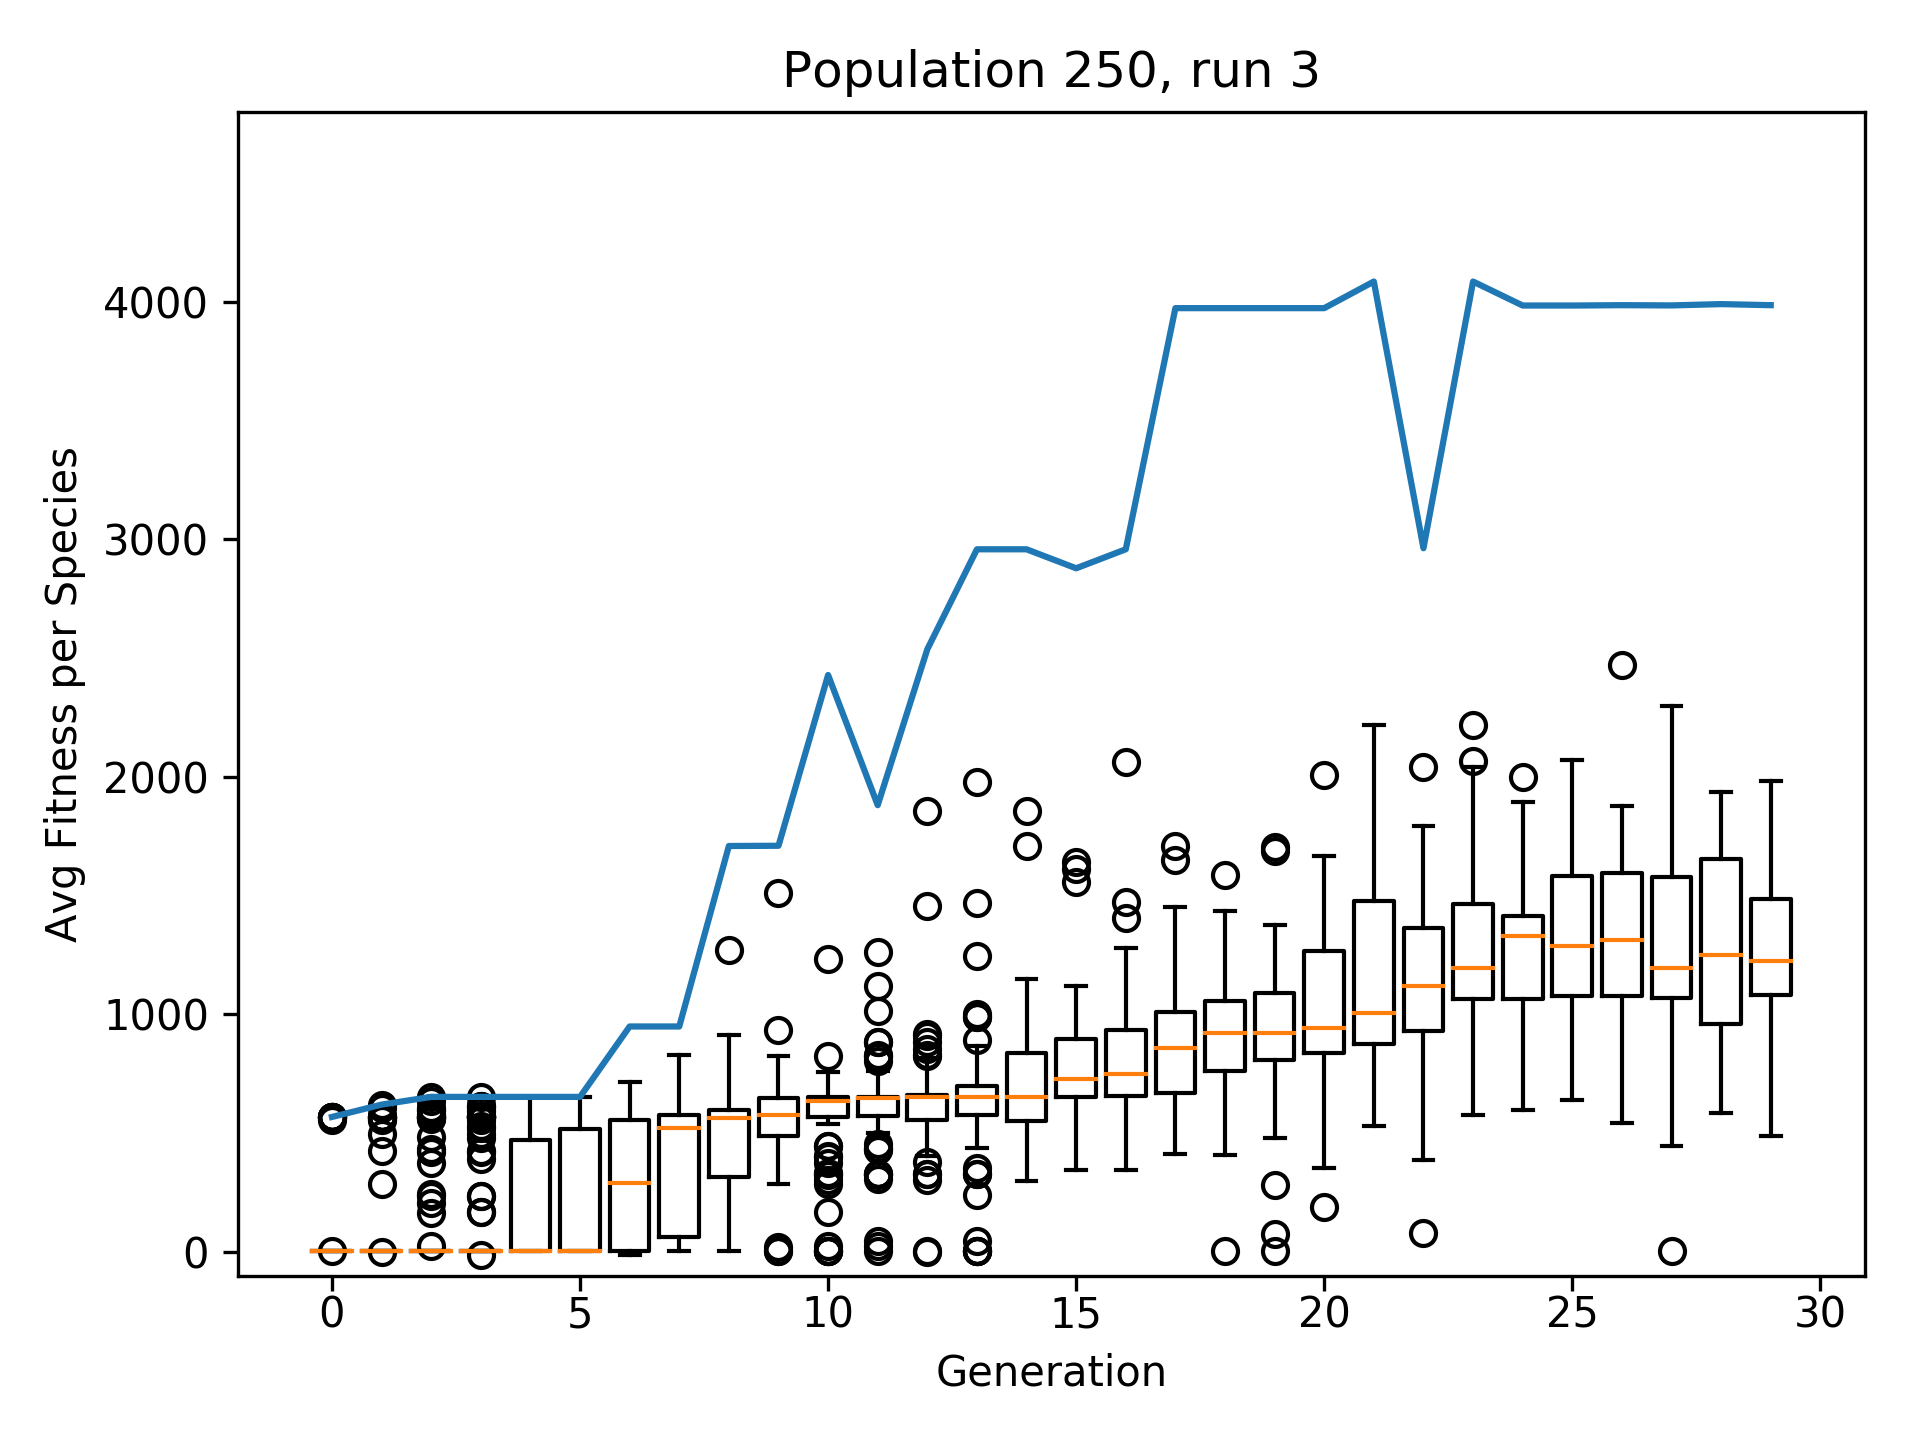
\includegraphics[width=1\textwidth]{graphics/mario/pop250_run3} % second figure itself
				\end{minipage}
				\caption{MarI/O Population 250}
				\label{fig:mario250}
			\end{figure}
			In figure \ref{fig:mario250} the population size is up to 250 in generation 0. In the first generation (Gen 0) 250 species are born with one genome each. The $average\_distance$ for this plot-runs is the biggest with approximately $1827$ when compared to the plot-runs with an initial population size of 10 and 50. In this plots no generations had to be skipped in order to portray a descriptive graph since the maximum generation count is 30 in plot-run 2 (25 generations in run 1 and 29 generations in run 3).\\
			Already in the 6th generation, on average only 94.8 species where left. At the end of generation 25 there where 31 species left on average. \\
			Compared to the other two population classes there are at least 7 times more species left at the end of the simulations which results in longer whiskers of the boxplot.The wiskers even contains bad starts with fitness-scores lower than 100 in plot-run 1 and 2. Interestingly the best runs are always exceptions after generation 6 (in plot-run 1 and 2 even earlier). \\
			Further it is to mention that the plots are rather uniform compared to the plots of population 10 and 50. Therefore the $average\_fitness\_increase$ has similar values with a low variance which are $133.25$ for generation 1, around $121.08$ for generation 2 and $113.95$ for generation 3. The $average\_regress$ is the lowest in plot-run 1 with $-5.87$ approximately. This is because the maximum value of the succeeding generation is smaller then the previous generation in only 4 cases. The other two plot-runs have an $average\_regress$ of approximately $-19.97$ in plot-run 2 and $-61.92$ in plot-run 3. All of the plot-runs reached the end of the level even thought plot-run 3 reached the end at generation 17, whereas plot-run 1 reached the end at generation 23 and plot-run 2 at generation 22.	
	
		\paragraph{Comparison of the results}
			\begin{table}[h]
				\centering
				\resizebox{\textwidth}{!}{
					\begin{tabular}[width=0.5\textwidth]{@{}ll|l|l|l|l@{}}
						\toprule
						{\Large MarI/O} & avg. runs /$\sigma$ 			& avg. fitness score /$\sigma$ 	& avg distance /$\sigma$ 	& avg. regress /$\sigma$ & avg. fitness increase /$\sigma$ 	\\ \midrule
						Population 10  	& 2828 /2055.44             	& 1231.42 /531.37      			& 1107.09 /534.5         	& -182.03 /144.01        & 10.6 /8.28             			\\
						Population 50  	& $4494.\overline{6}$ /176.09	& 960.96 /321.34       			& 1405.96 /664.75        	& -105.56 /86.01         & 30 /10.78              			\\
						Population 250 	& 5329 /656.74               	& 776.31 /57.88        			& 1826.32 /81.79        	& -29.25 /29.16          & 122.76 /9.76           			\\ \bottomrule
					\end{tabular}
				}
				\caption{MarI/O Population Comparison Overview}
				\label{tab:mario}
			\end{table}
			\todo{Differences and similarities between runs in graph} \\
			In order to compare the results, 5 distinct values (see table \ref{tab:mario}) of the plot-runs where calculated, as three of them were introduced in more detail earlier in this section \ref{par:mario10}. The first observations indicate that the average fitness score of each generation drops when establishing a bigger initial population. However the standard deviation tend to drop as well. \\
			Also the distance of the median of the species to the best run of the generation seam to become greater with a greater population count in generation 0. However, the average regress (if present) becomes lower with bigger population sizes and fewer generations, as well as it's deviation. Since there are fewer generations in the simulations with an initial population of 250 and these simulations having similar achievements, the average fitness increase is higher than in the other two simulation classes. The standard deviation of the average fitness increase is relatively similar.\\
			It is interesting to see how the fitness increase compares to the average distance value. Even thought the fitness increase of population class 250 is much higher than the fitness increase of population class 10, the distance remains largs which indicates that the majority of runs stayed low and the average score of population class 10 is higher than in the other two population classes. Still the other two classes remained more stable when taking the average regress into account. \\
			Another interesting point of view is the reaching of the end of the level (the goal). In all population classes the goal was reached even thought population class 1 and 2 didn't reach the goal in one plot-run each. Population 10 reached the goal in the first $24.48\%$ on average, only including the cases where the goal was reached. Population 50 reached the goal in the first $40,24\%$ on average and population class 250 in the first $69,47\%$.\\
			To summarize the results roughly it can be said that an initial population size of 10 promises faster and better results in an complex environment like Super Mario World, however more stability can be reached when increasing the initial population size.
		
	% FLAPPY BIRD ###############################################################
	
	\section{Machine Learning Flappy Bird}
		\label{sec:analysis:flappy}
		\todo{change this title}
		
		\begin{figure}[h]
			\centering
			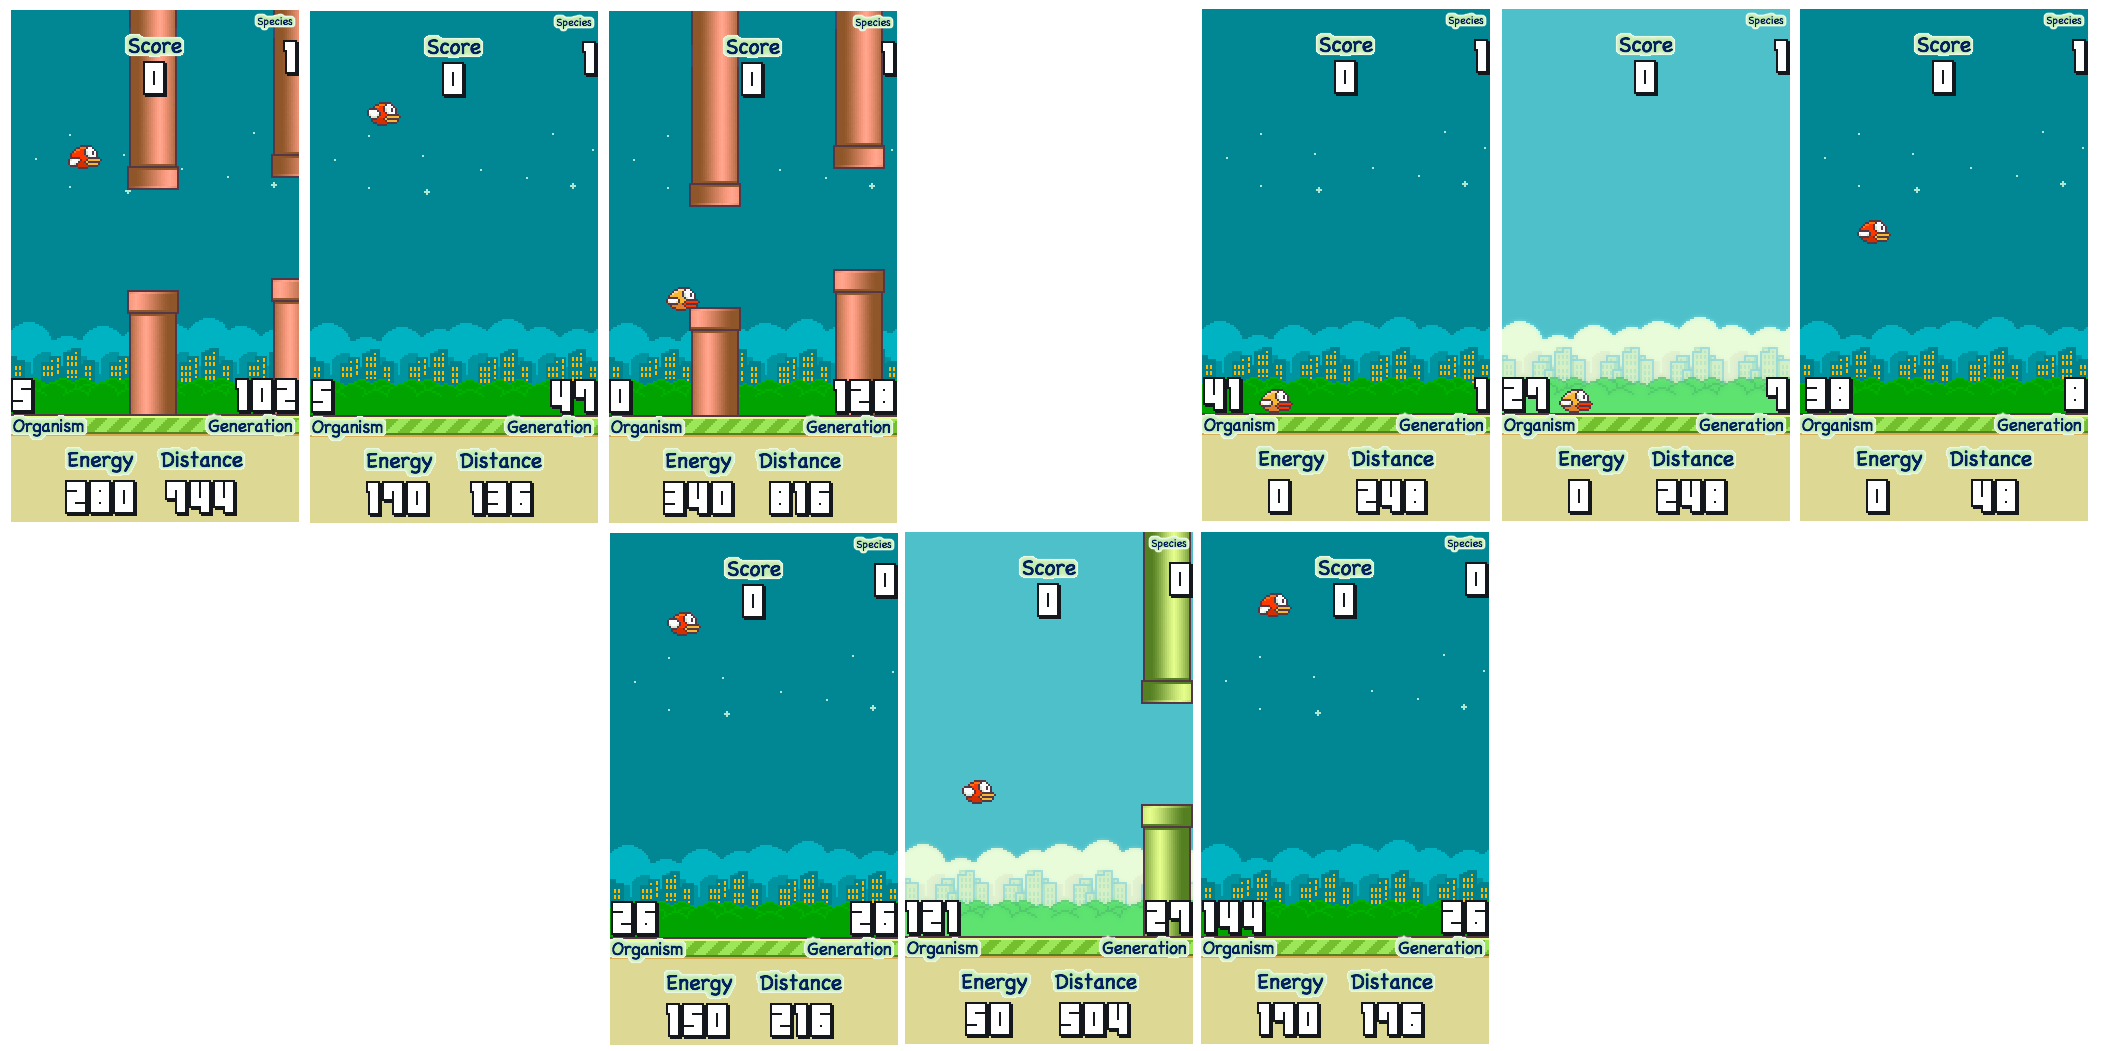
\includegraphics[width=1\textwidth]{graphics/flappy/flappy_sim_s1}
			\caption{Flappy Birds simulation}
			\label{fig:flappy}
		\end{figure}
		
		\begin{enumerate}
			\item explanation of environment and expectations
			\item fitnessfunction, formlar?
			\item explanation of graph of population (10, 50, 250) averaged on generations (30 generations evenly choosen [equal spaces between generation numbers])  (abstract explanation)
			\item check if expectations of marI/O can confirm
			\item huge difference between best runs and majority of runs (extreme luck), => double graph
			\item Differences between runs 
			\item unexpectedly bad results
			\item => Neat vs other machine learning
			\begin{enumerate}
				\item Differences between runs (lucky runs with 4th champion generation)
			\end{enumerate}
		\end{enumerate}
		
		\paragraph{Population 10 / Generation 500}
			\begin{figure}[h!]
				\centering
				\begin{minipage}{0.33\textwidth}
					\centering
					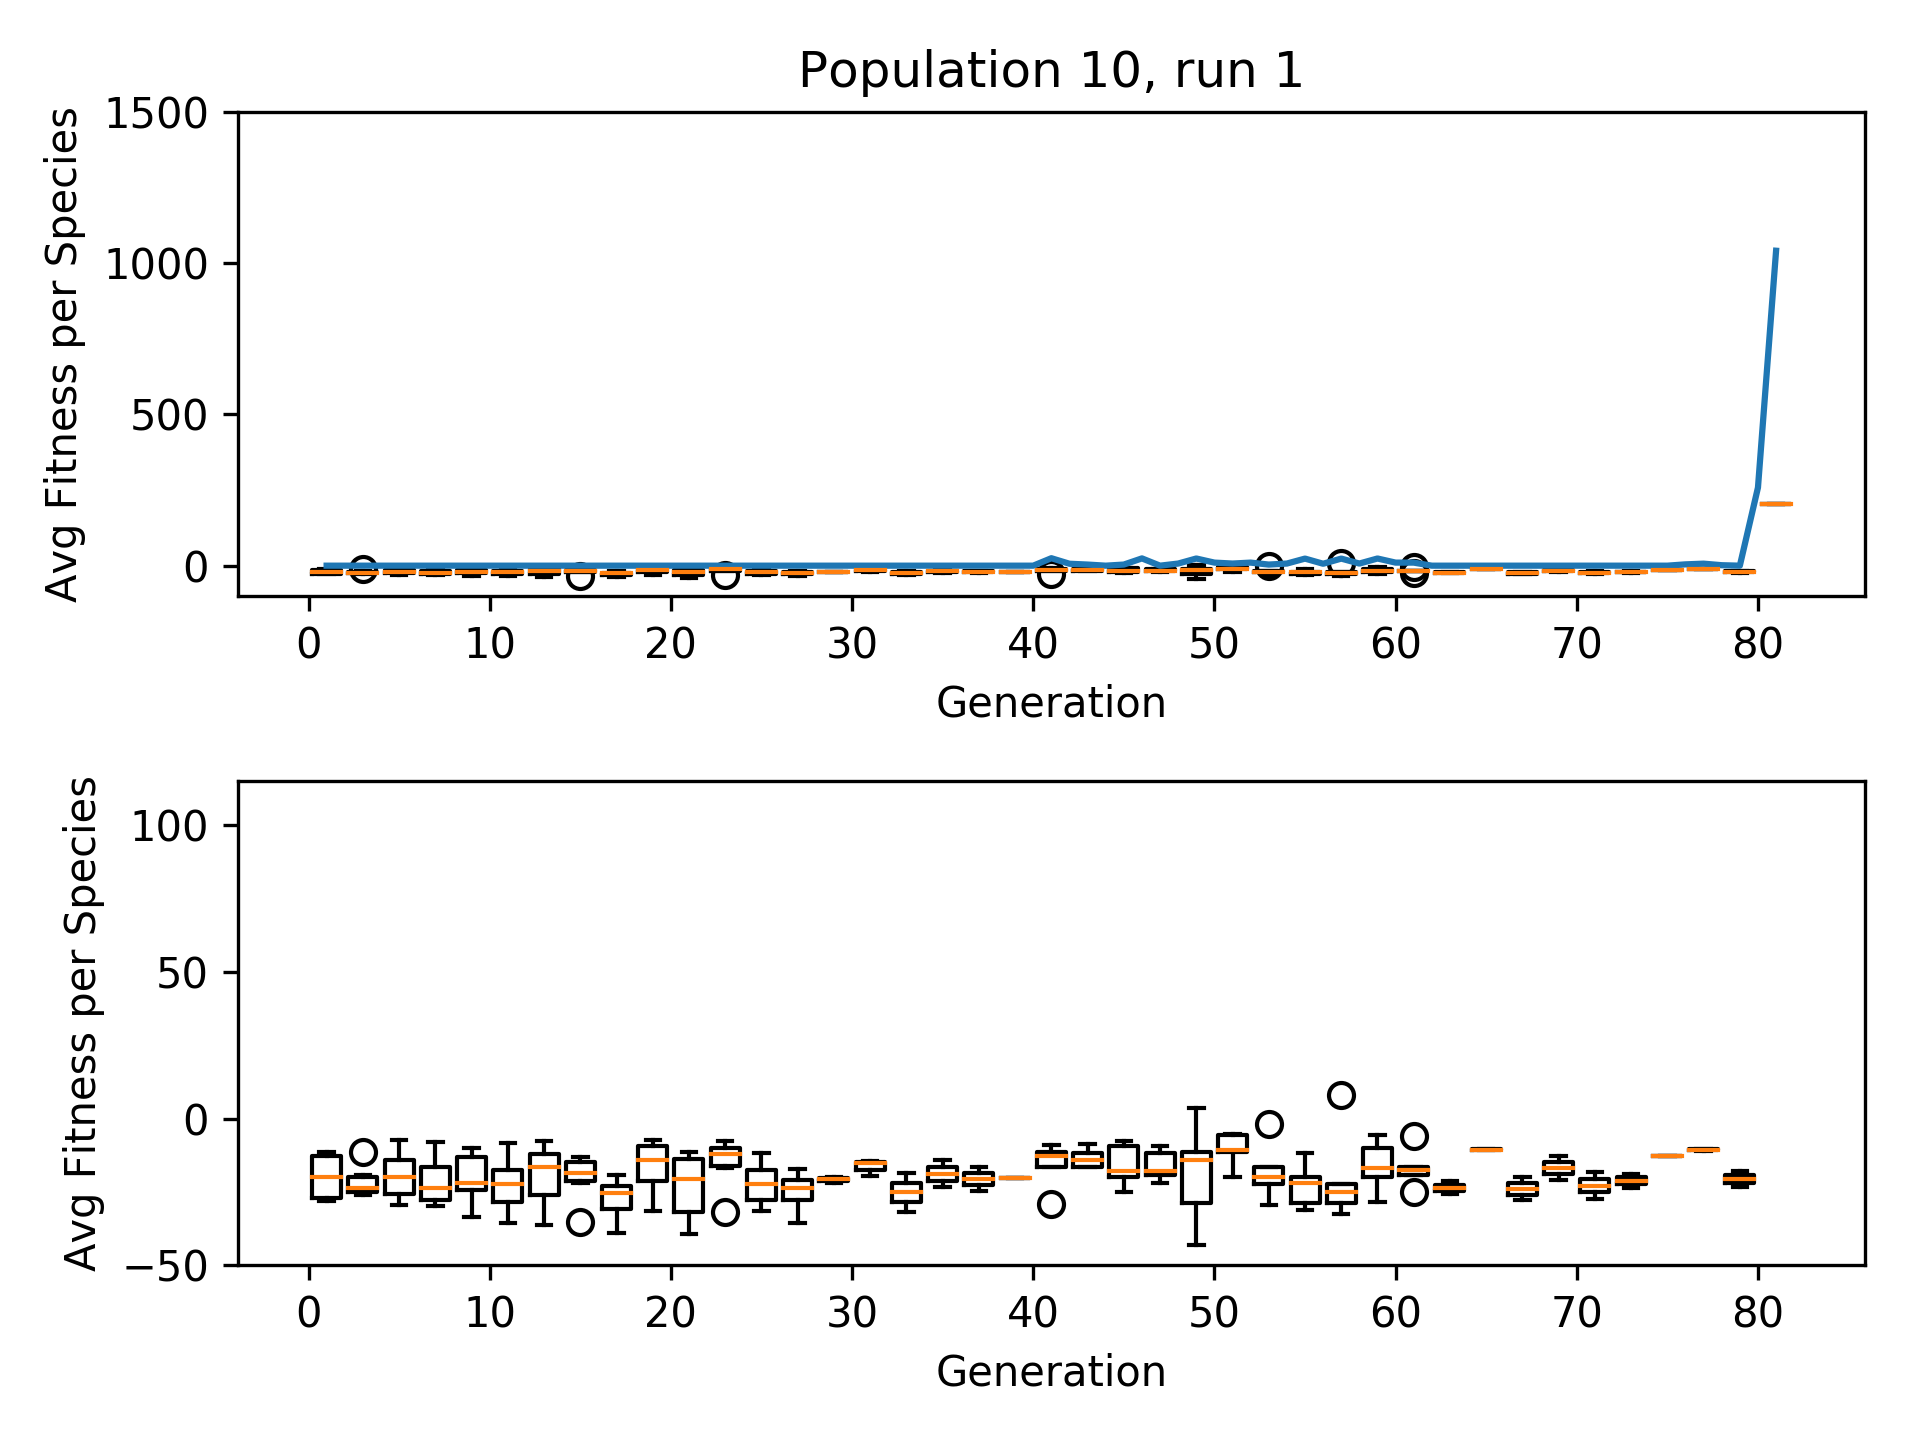
\includegraphics[width=1\textwidth]{graphics/flappy/pop10_run1} % first figure itself
				\end{minipage}\hfill
				\begin{minipage}{0.33\textwidth}
					\centering
					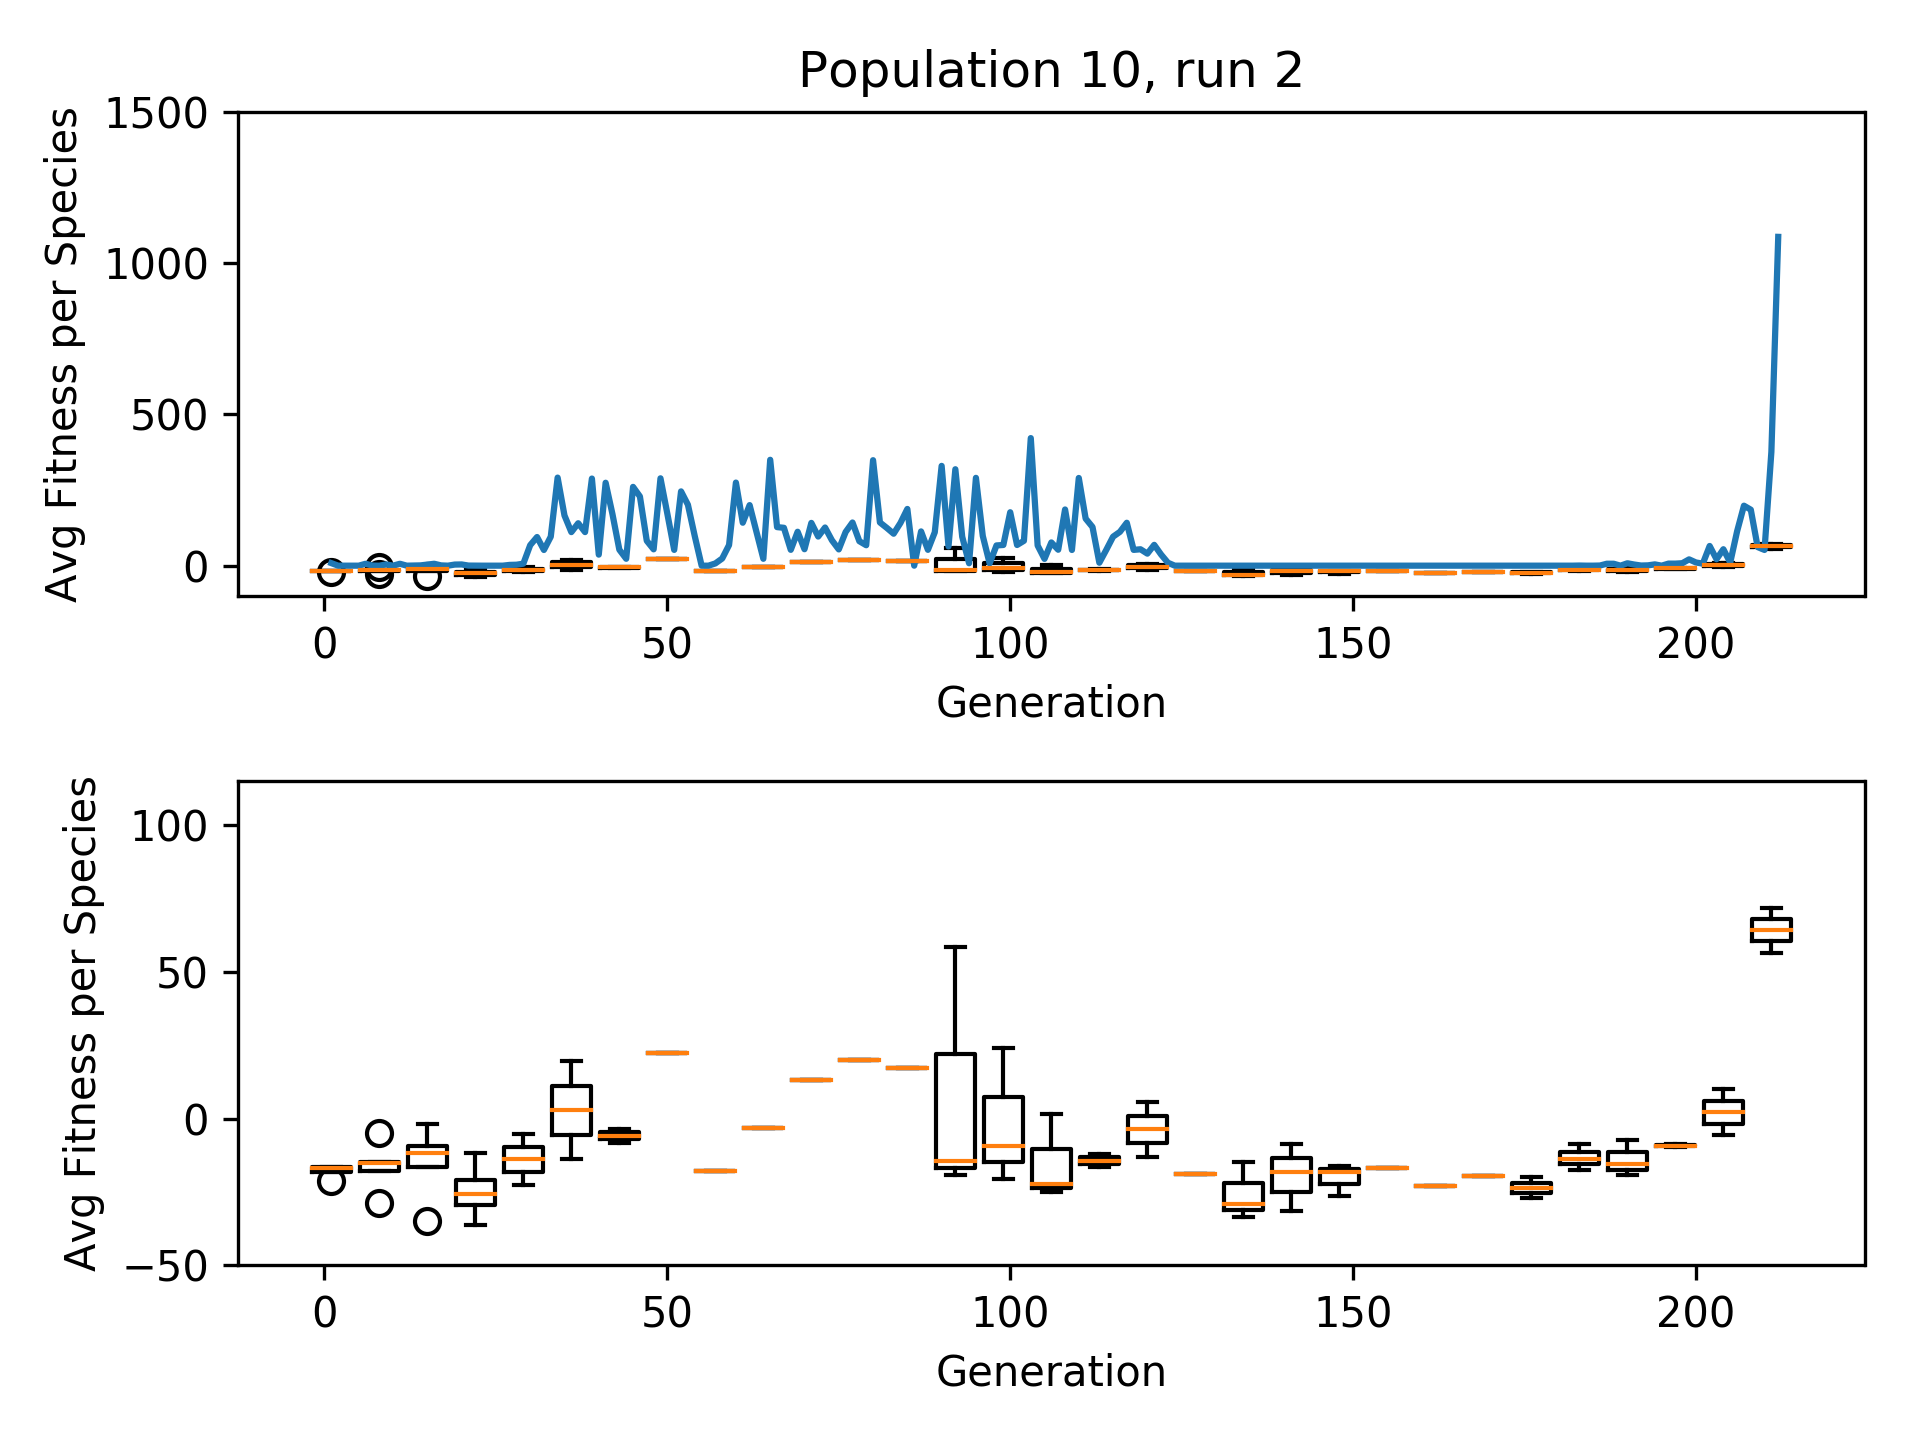
\includegraphics[width=1\textwidth]{graphics/flappy/pop10_run2} % second figure itself
				\end{minipage}
				\begin{minipage}{0.33\textwidth}
					\centering
					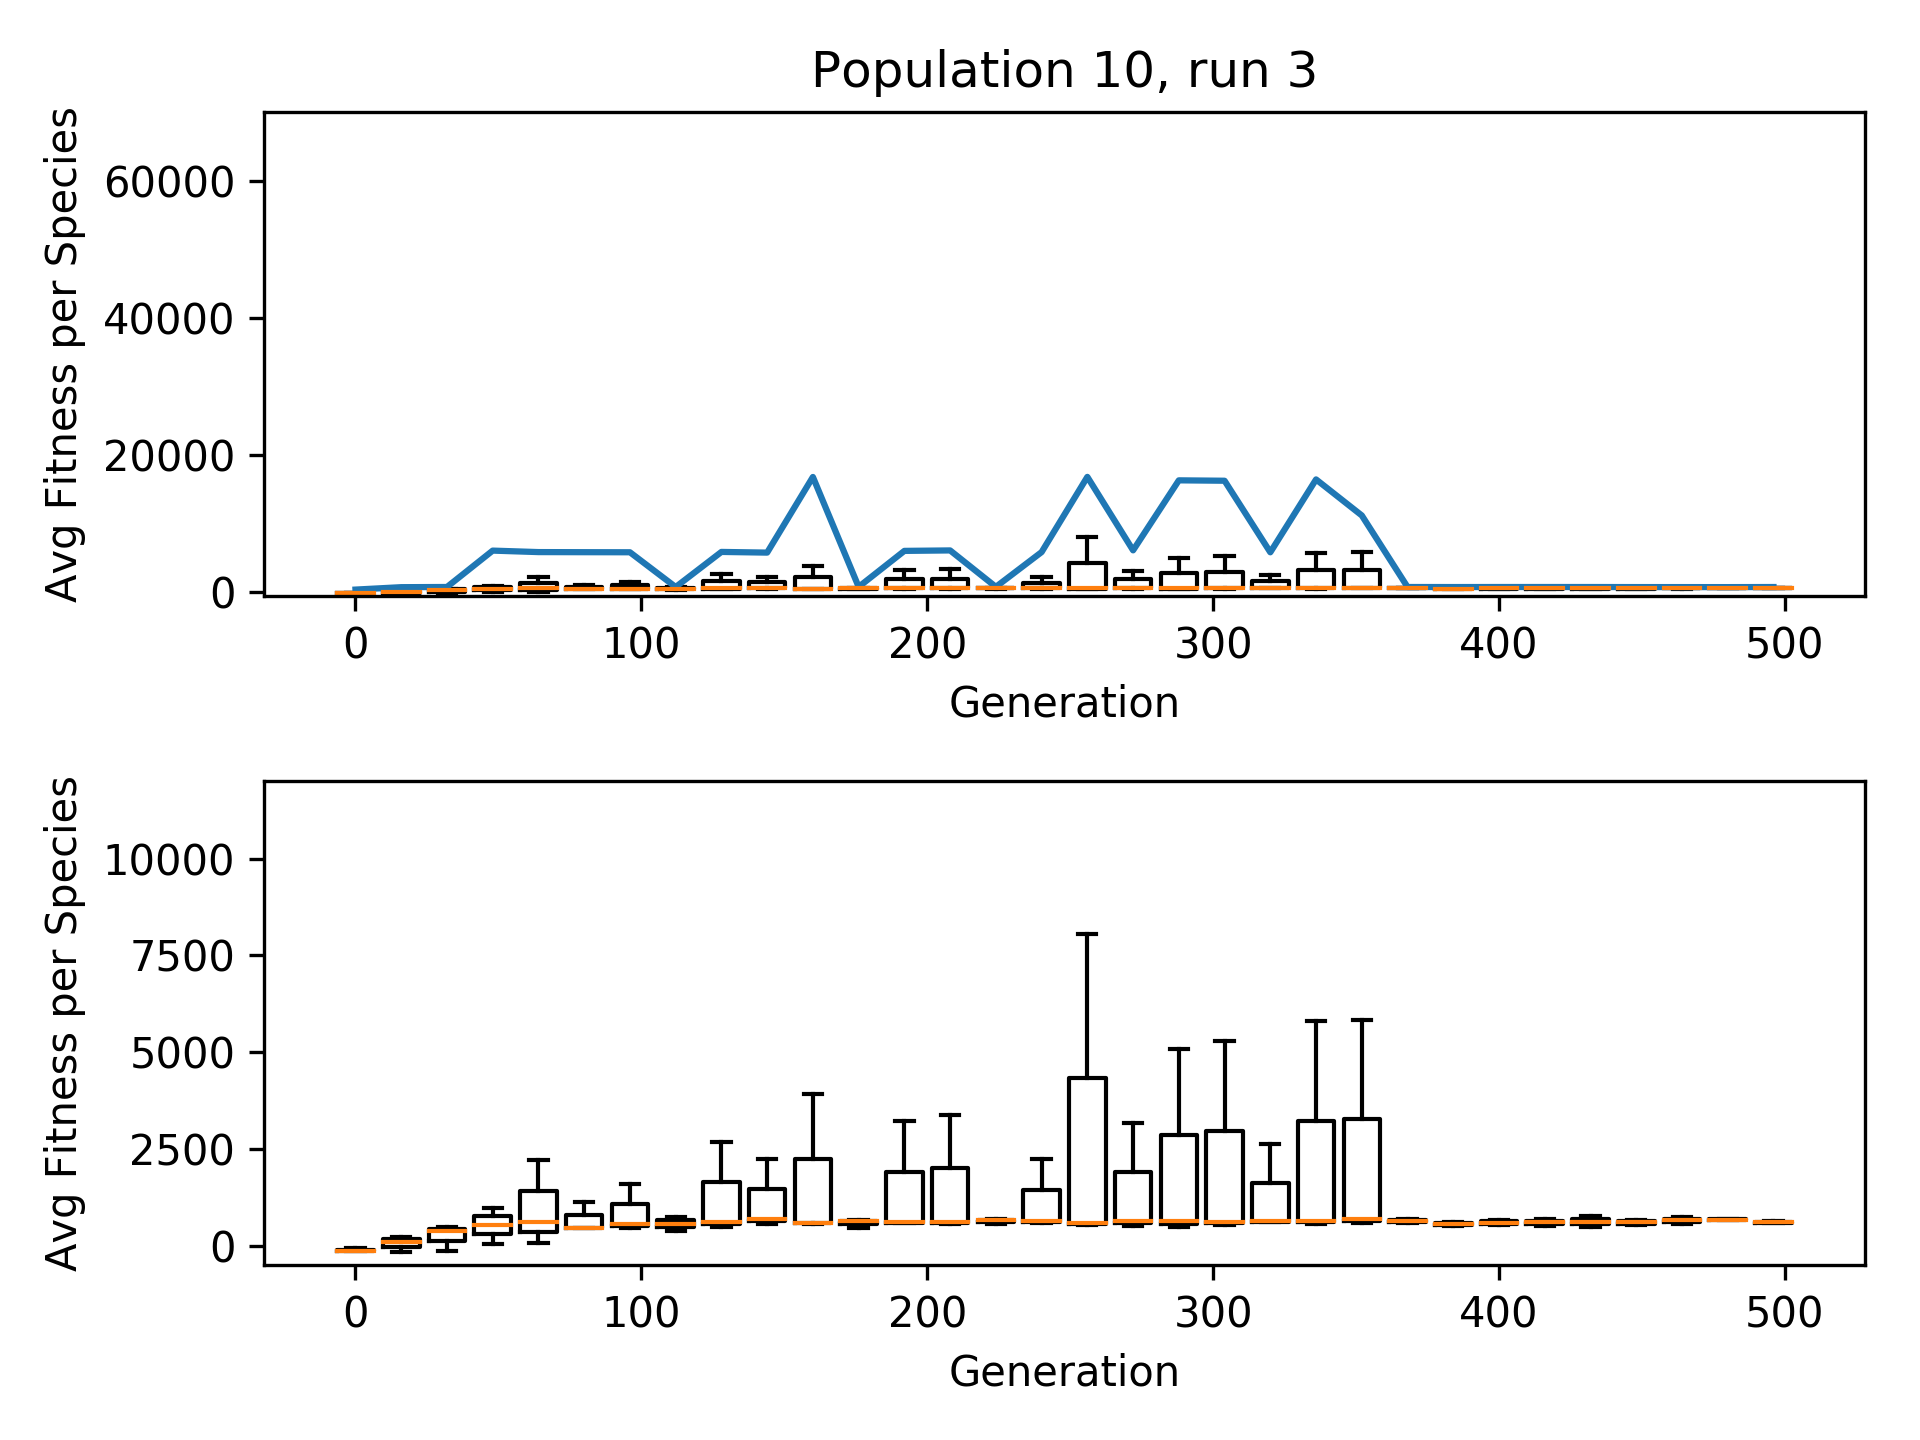
\includegraphics[width=1\textwidth]{graphics/flappy/pop10_run3} % second figure itself
				\end{minipage}
				\caption{Flappy Bird Population 10}
			\end{figure}
		
		\paragraph{Population 50 / Generation 100}
			a
%			\begin{figure}[h]
%				\centering
%				\begin{minipage}{0.33\textwidth}
%					\centering
%					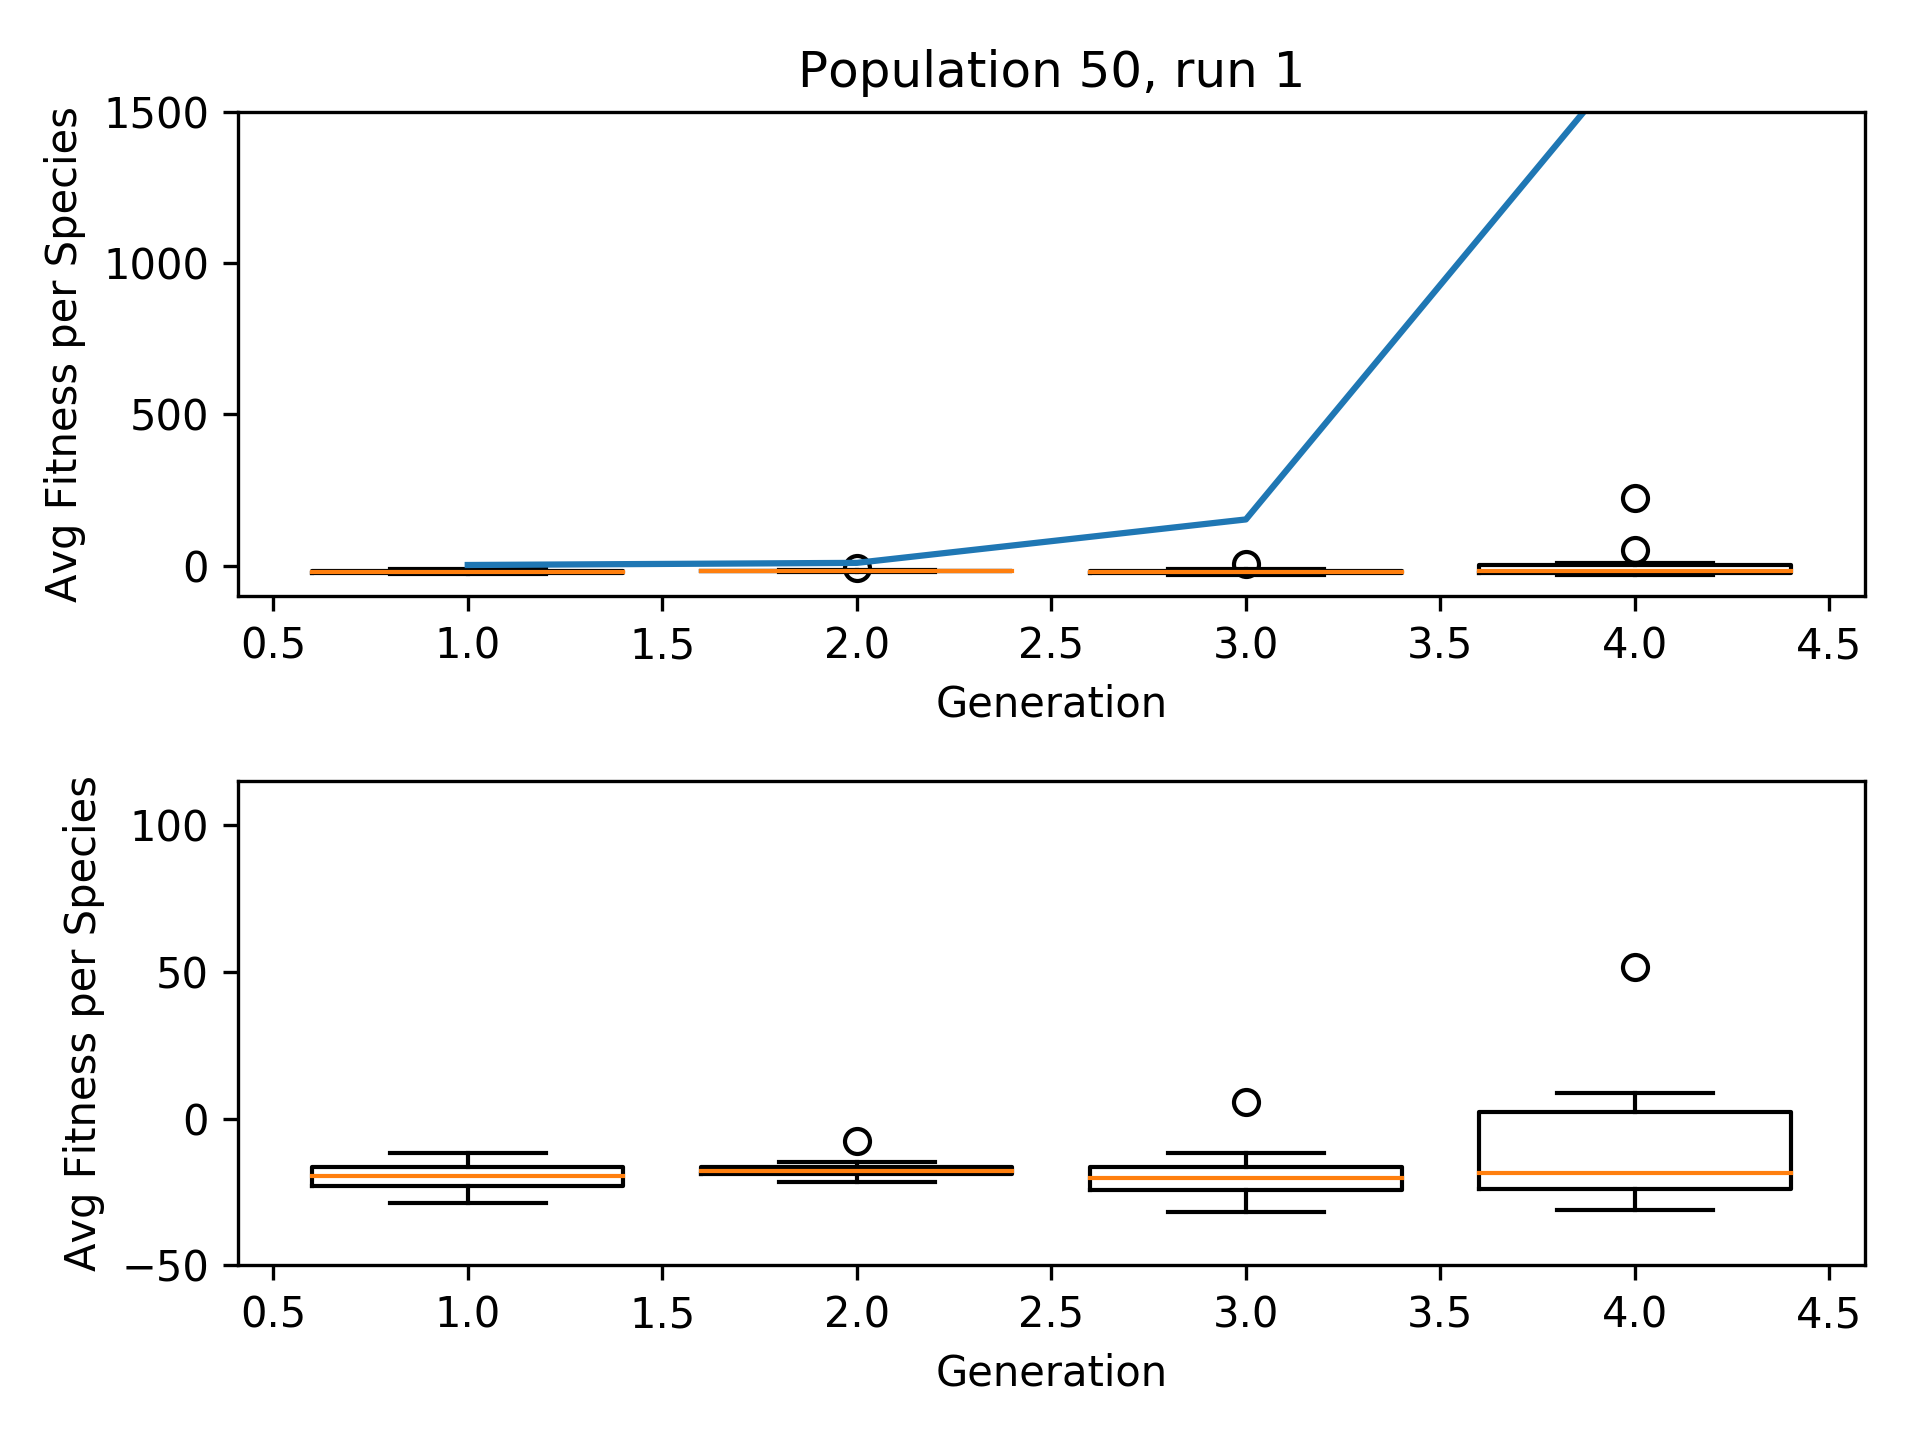
\includegraphics[width=1\textwidth]{graphics/flappy/pop50_run1} % first figure itself
%				\end{minipage}\hfill
%				\begin{minipage}{0.33\textwidth}
%					\centering
%					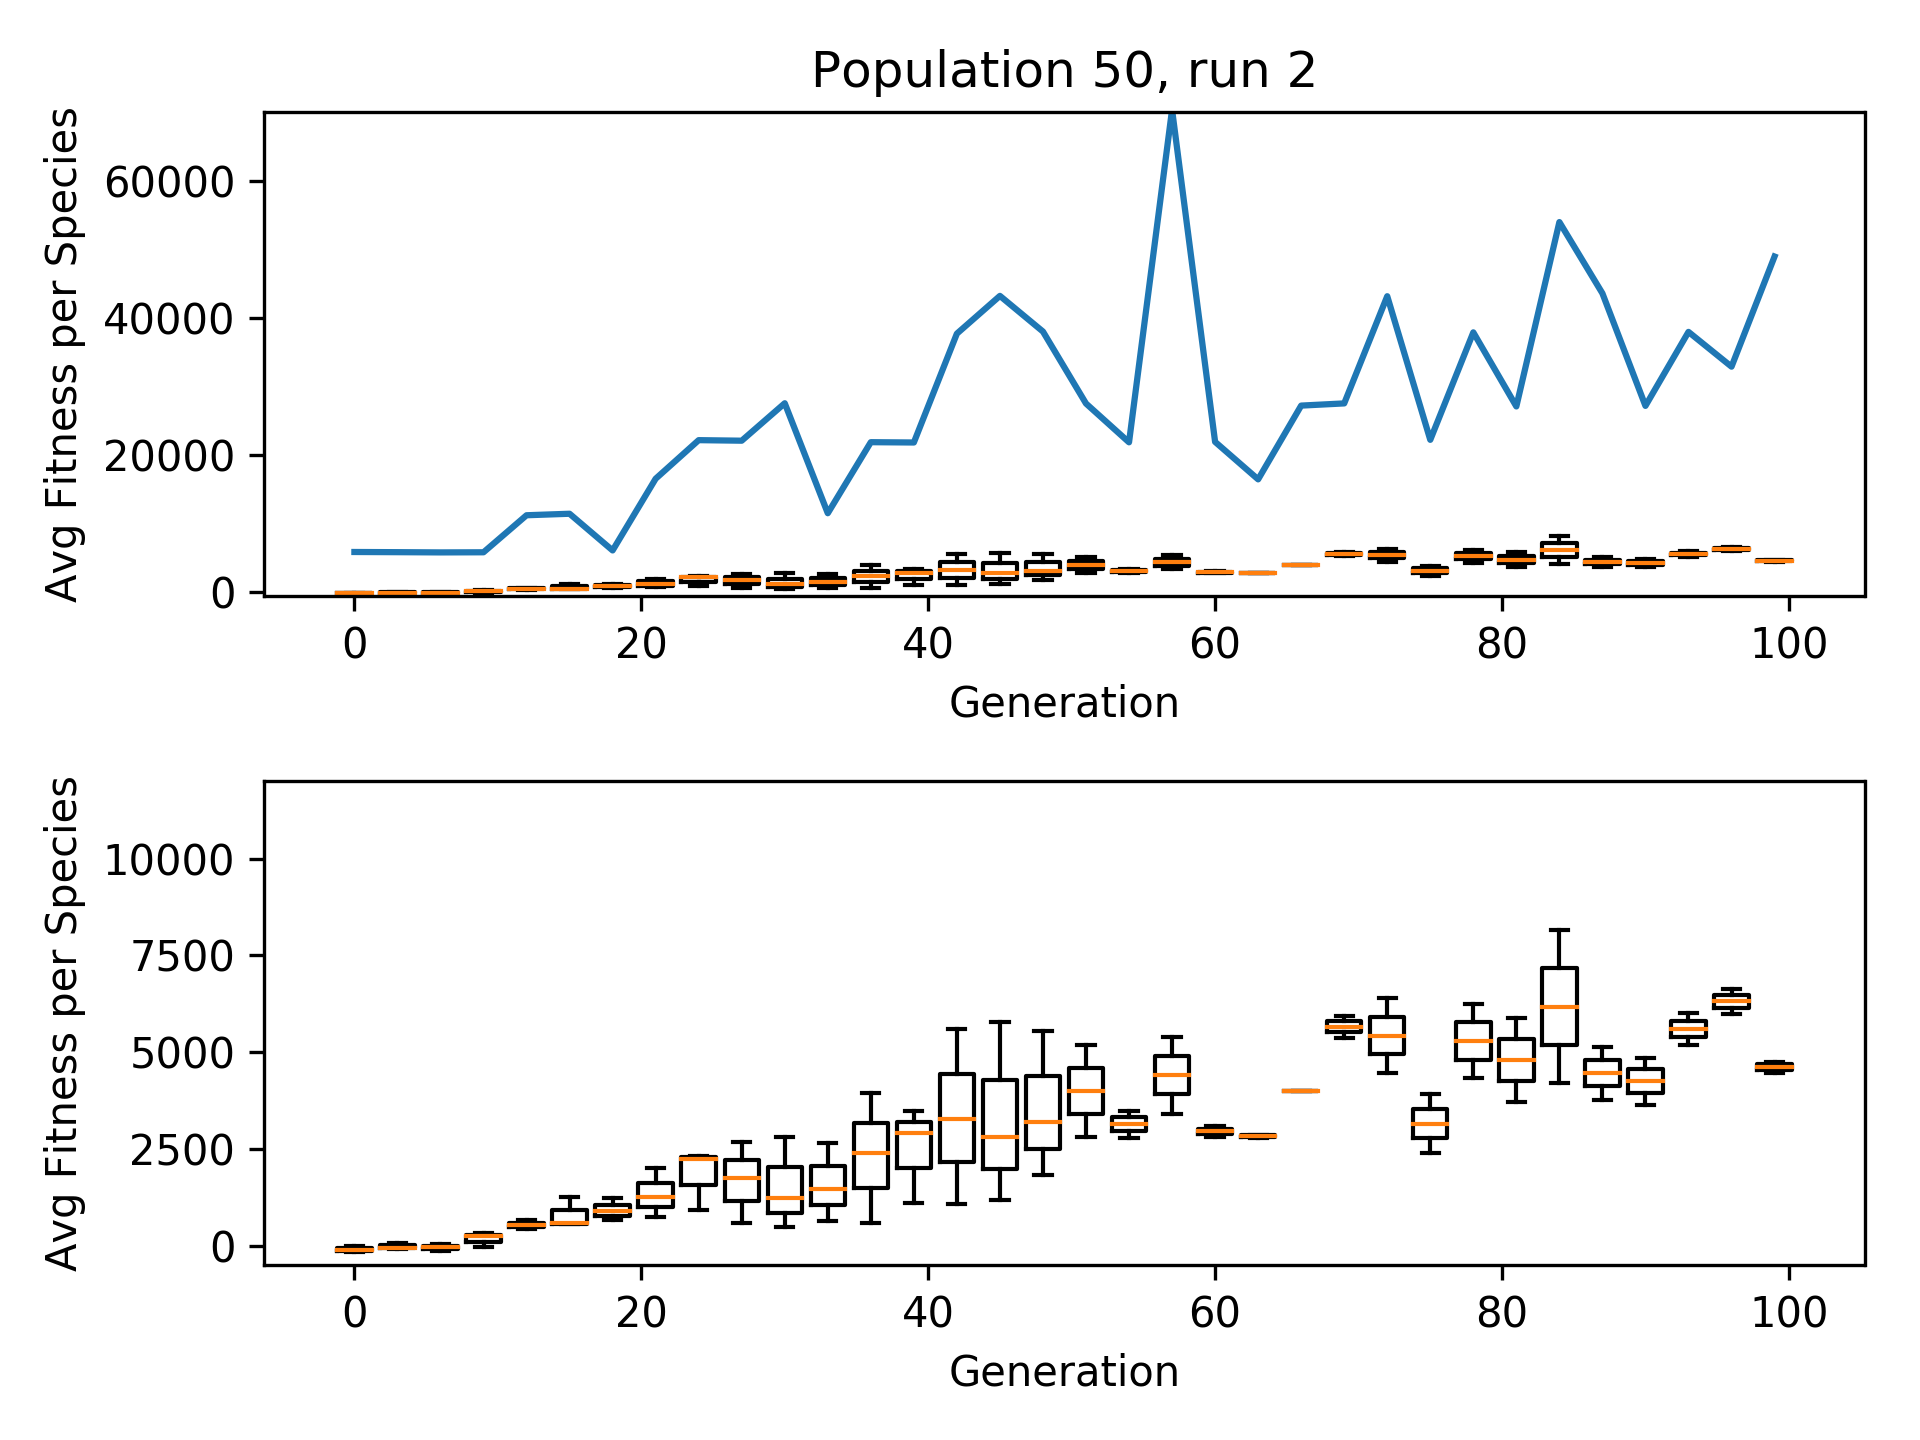
\includegraphics[width=1\textwidth]{graphics/flappy/pop50_run2} % second figure itself
%				\end{minipage}
%				\begin{minipage}{0.33\textwidth}
%					\centering
%					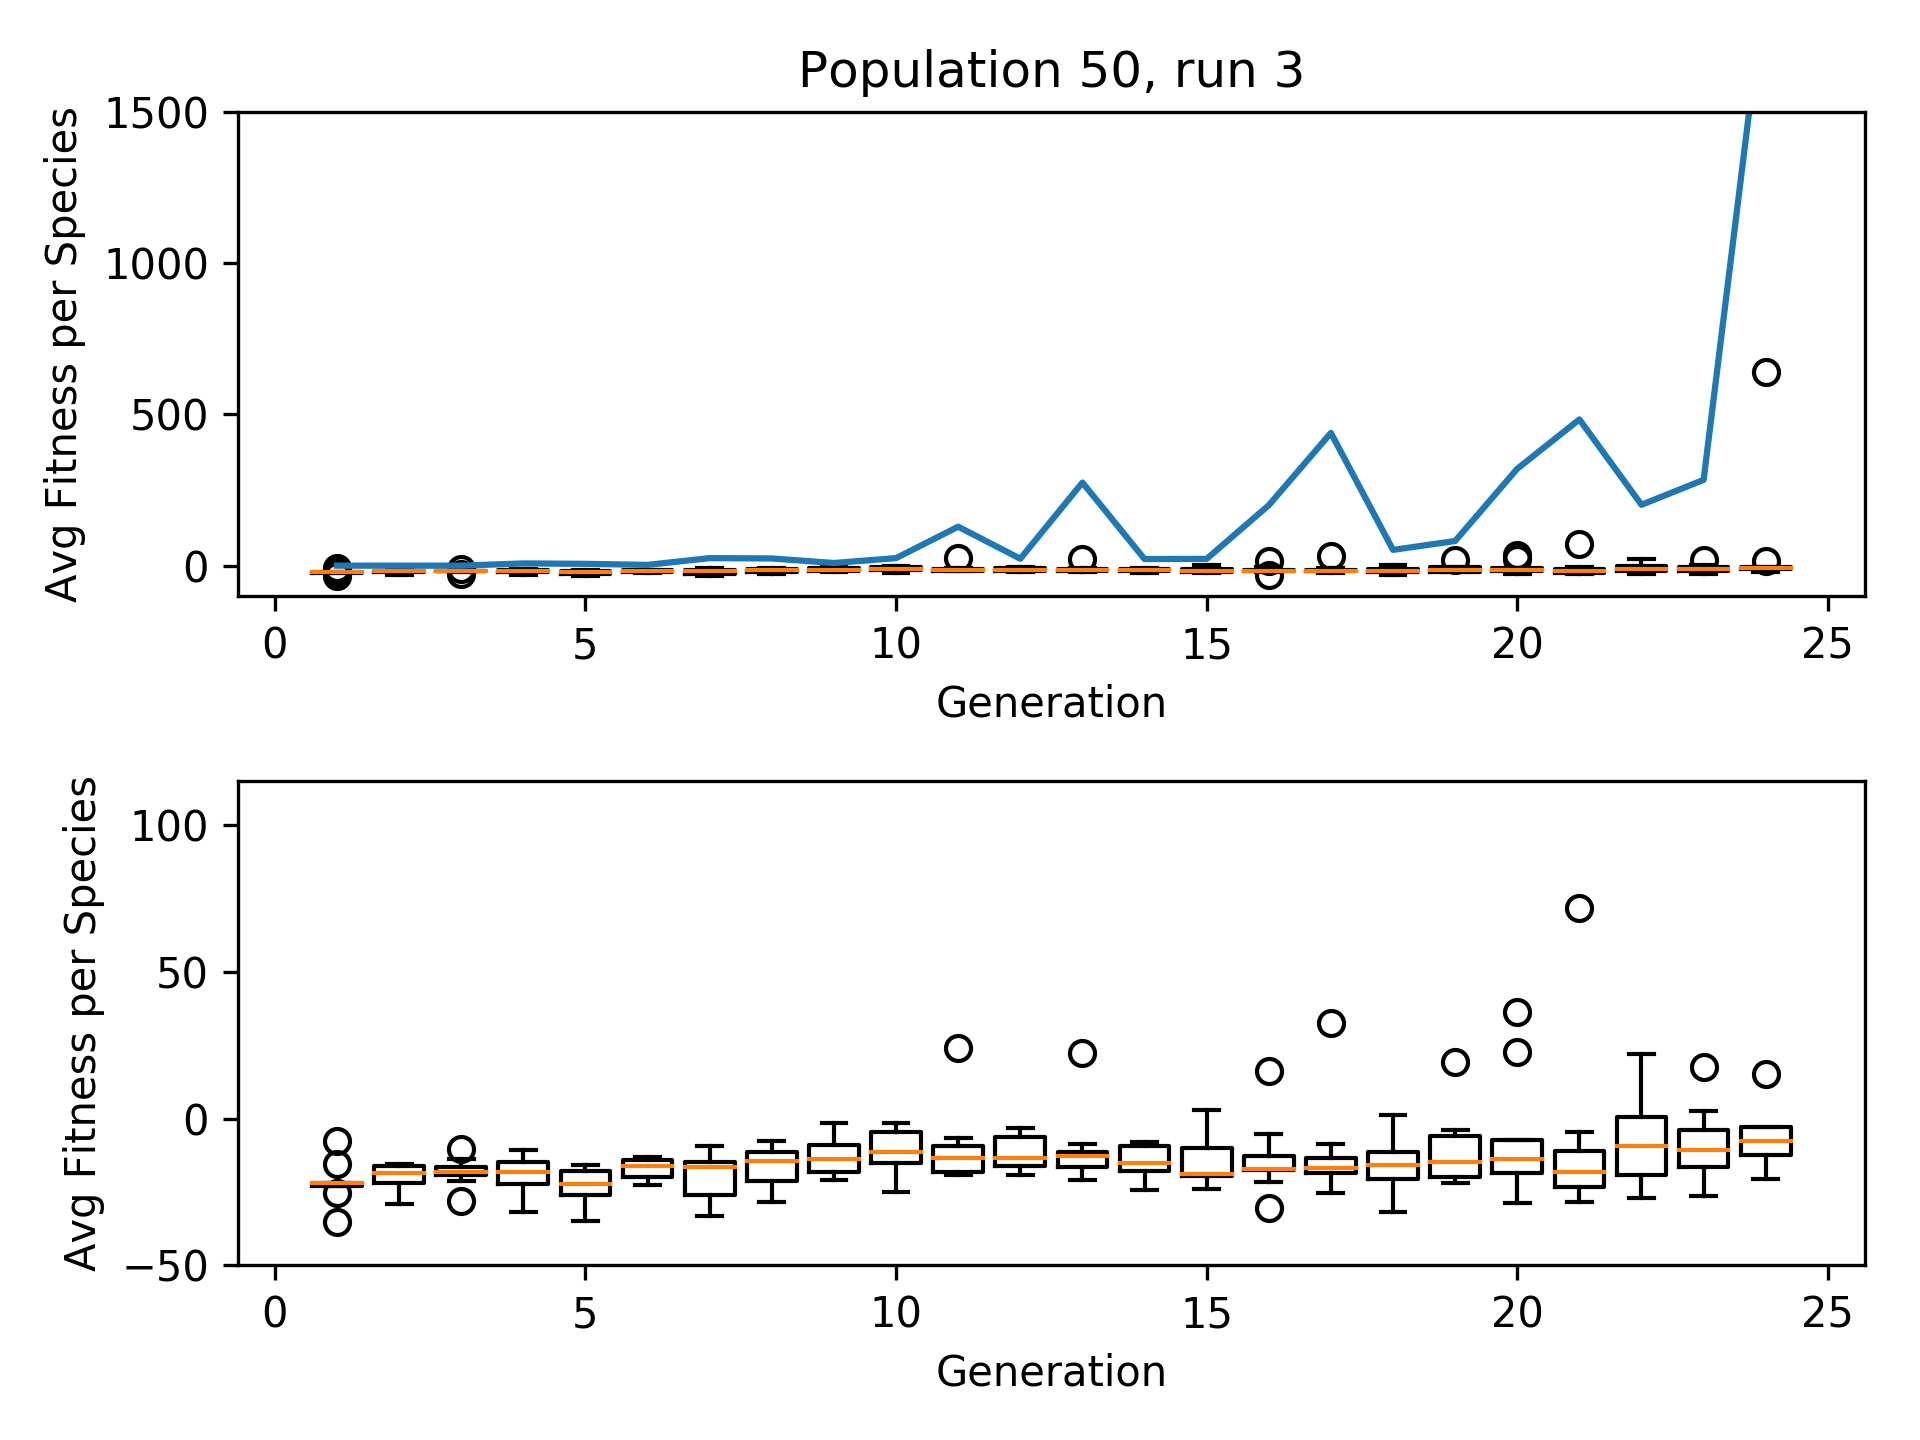
\includegraphics[width=1\textwidth]{graphics/flappy/pop50_run3} % second figure itself
%				\end{minipage}
%				\caption{Flappy Bird Population 50}
%			\end{figure}
		
		\paragraph{Population 250 / Generation 30}
		
			\begin{enumerate}
				\item best runs are exceptions (outside of whiskers)
			\end{enumerate}
			
%			\begin{figure}[h]
%				\centering
%				\begin{minipage}{0.33\textwidth}
%					\centering
%					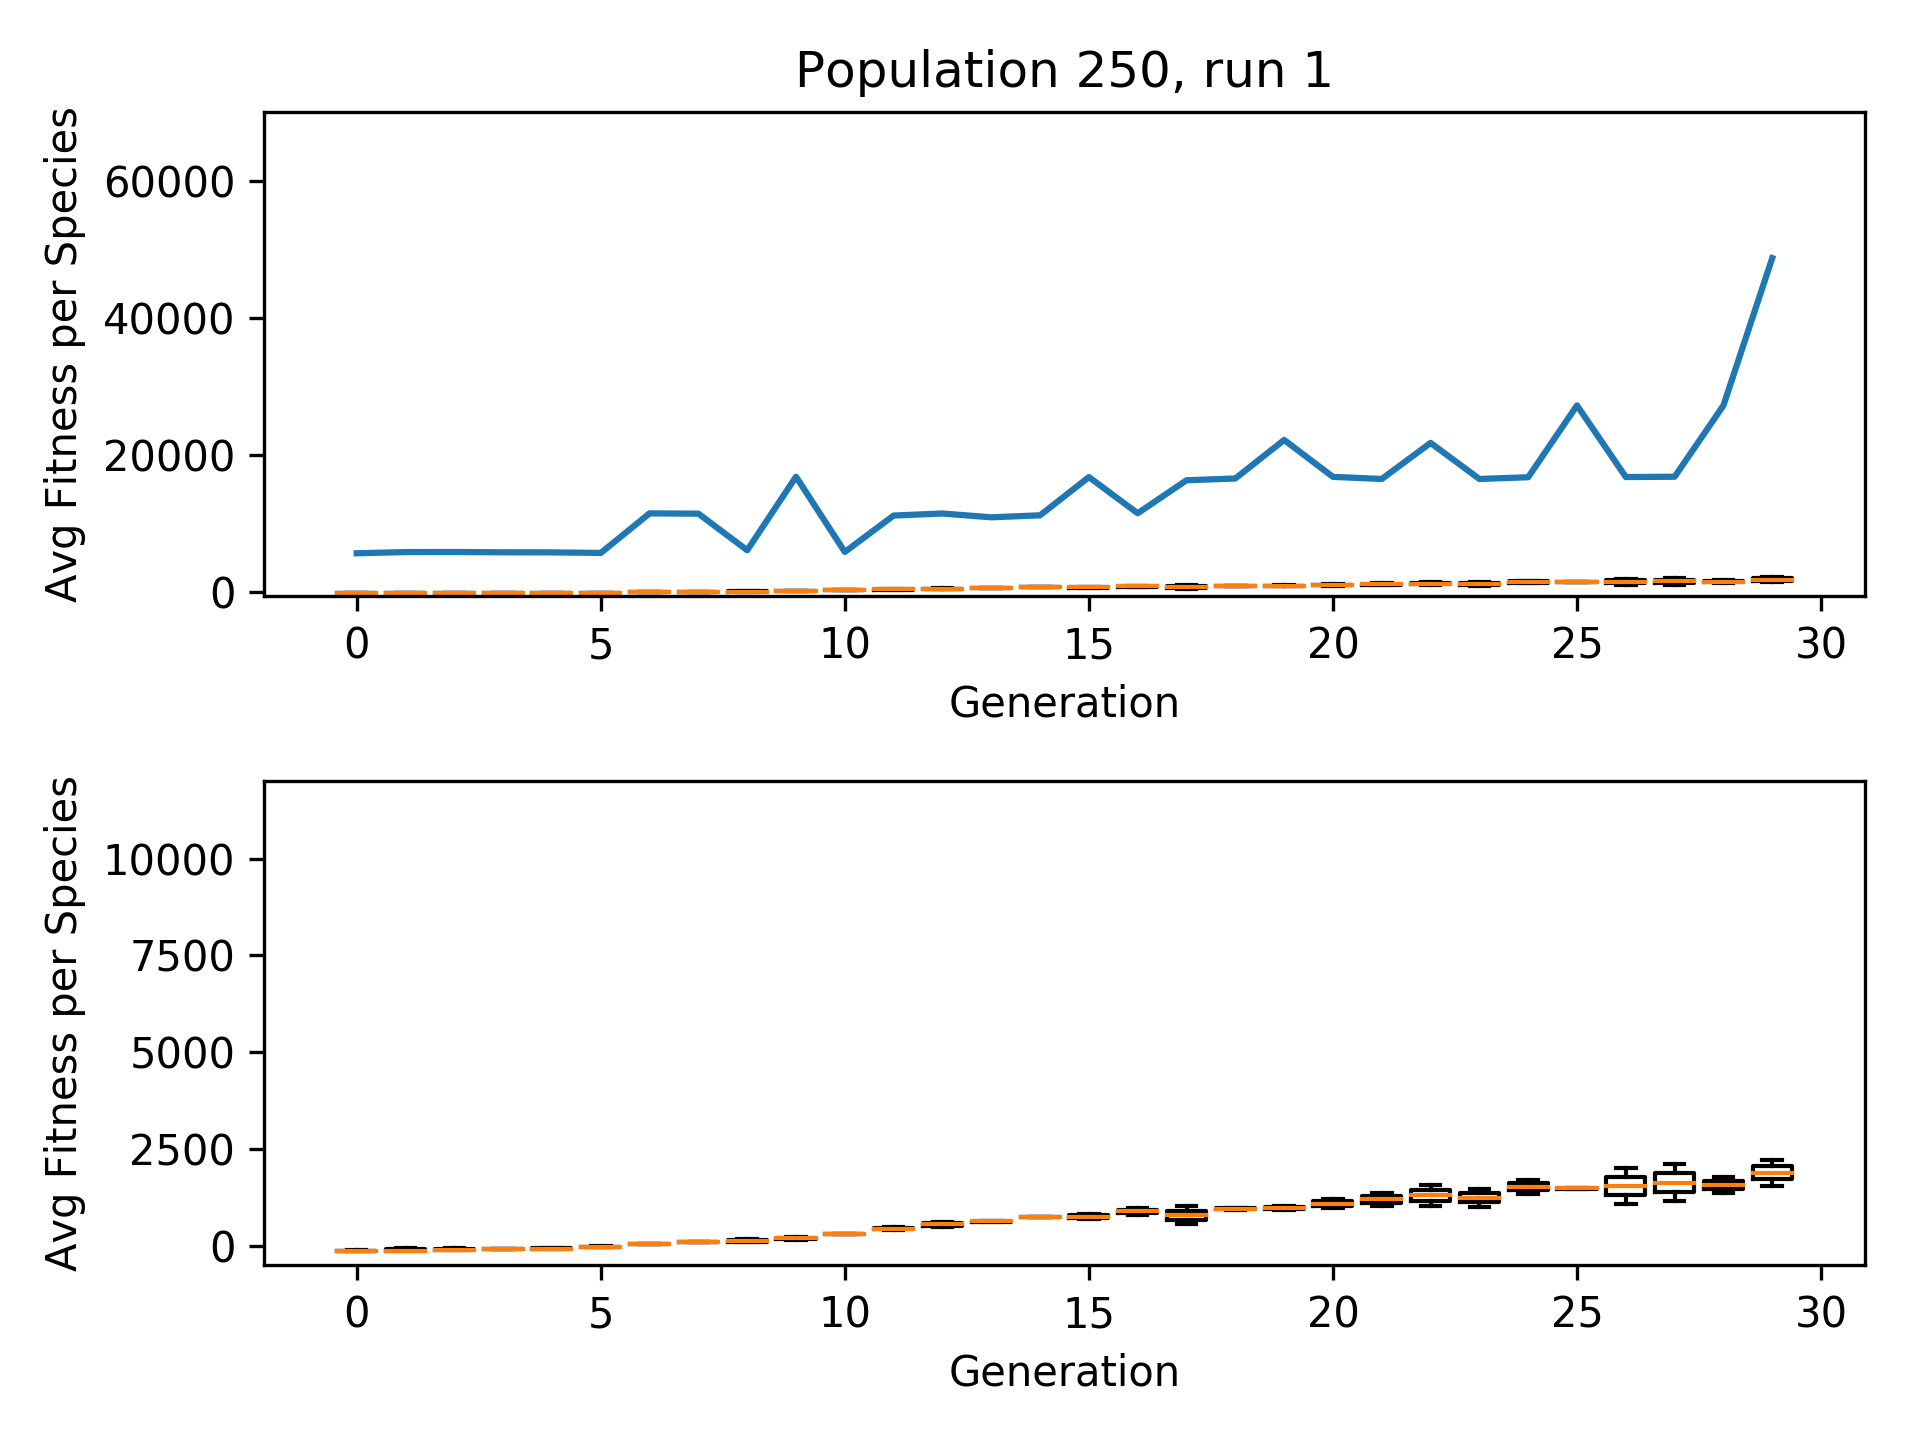
\includegraphics[width=1\textwidth]{graphics/flappy/pop250_run1} % first figure itself
%				\end{minipage}\hfill
%				\begin{minipage}{0.33\textwidth}
%					\centering
%					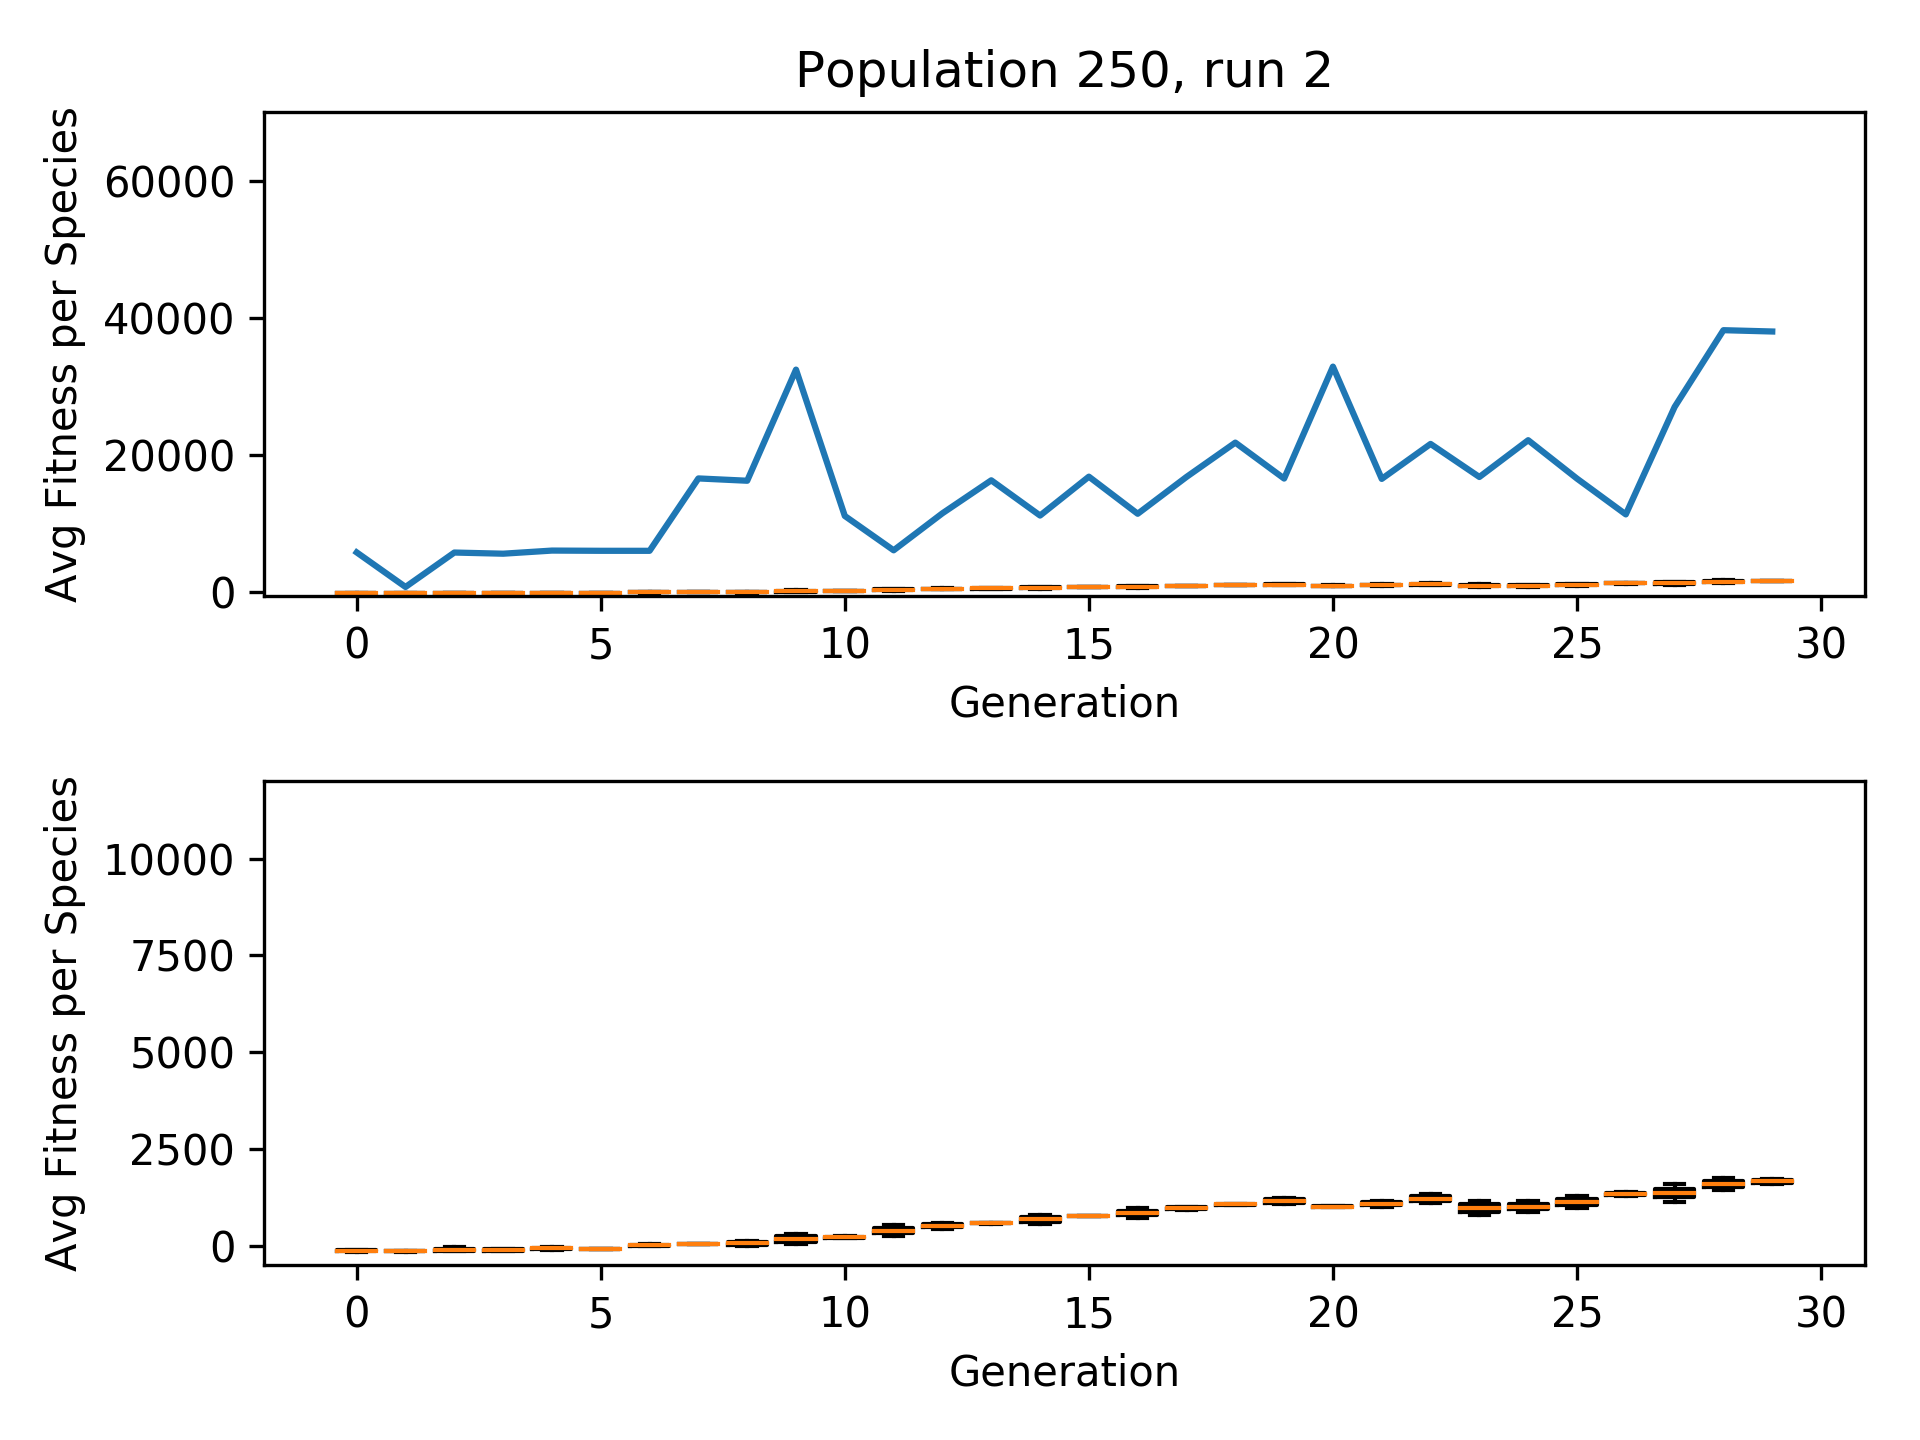
\includegraphics[width=1\textwidth]{graphics/flappy/pop250_run2} % second figure itself
%				\end{minipage}
%				\begin{minipage}{0.33\textwidth}
%					\centering
%					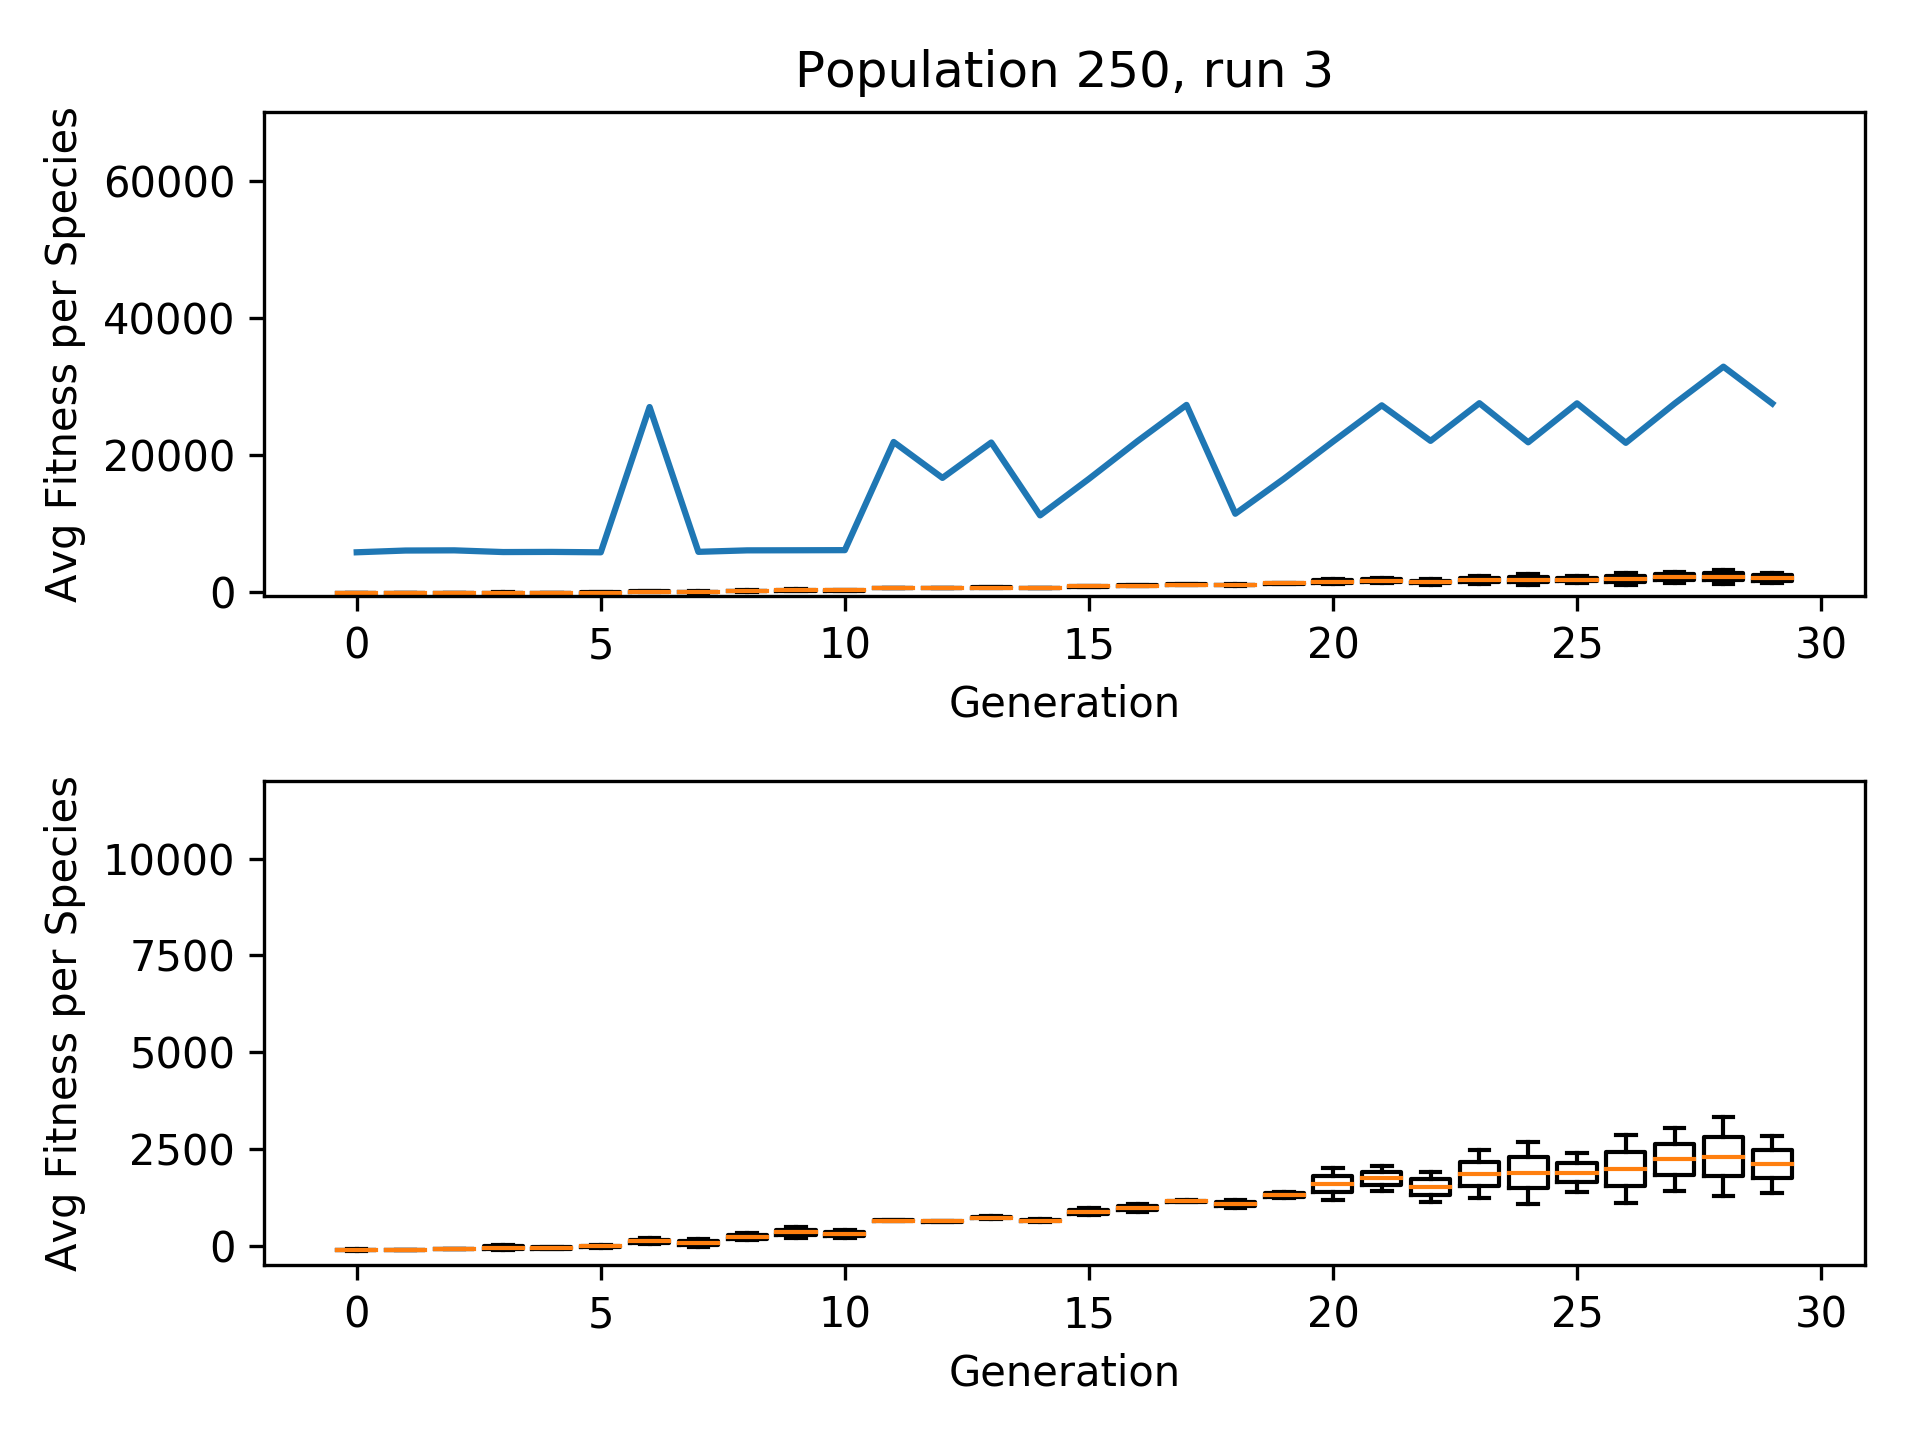
\includegraphics[width=1\textwidth]{graphics/flappy/pop250_run3} % second figure itself
%				\end{minipage}
%				\caption{Flappy Bird Population 250}
%			\end{figure}
		
		\paragraph{Comparison of the results}
			\begin{table}[h]
				\centering
				\resizebox{\textwidth}{!}{
					\begin{tabular}[width=0.5\textwidth]{@{}ll|l|l|l|l@{}}
						\toprule
						{\Large MarI/O} & avg. runs /$\sigma$ 			& avg. fitness score /$\sigma$ 	& avg distance /$\sigma$ 	& avg. regress /$\sigma$ & avg. fitness increase /$\sigma$ 	\\ \midrule
						Population 10  	& 2828 /2055.44             	& 1231.42 /531.37      			& 1107.09 /534.5         	& -182.03 /144.01        & 10.6 /8.28             			\\
						Population 50  	& $4494.\overline{6}$ /176.09	& 960.96 /321.34       			& 1405.96 /664.75        	& -105.56 /86.01         & 30 /10.78              			\\
						Population 250 	& 5329 /656.74               	& 776.31 /57.88        			& 1826.32 /81.79        	& -29.25 /29.16          & 122.76 /9.76           			\\ \bottomrule
					\end{tabular}
				}
				\caption{MarI/O Population Comparison Overview}
				\label{tab:mario}
			\end{table}
		
		\subsection{Plain Machine learning flappy bird}
			\begin{enumerate}
				\item better results
				\item multi simulation made it easier
				\item easy algorithm for easy environment might be explanation for better results
			\end{enumerate}
			\paragraph{Comparison to \gls{neat} results}
	
	
	\section{Conclusion}
		\label{sec:analysis:conclusion}
		\begin{enumerate}
			\item Population sizes smart? (10, 50, 250)
			\item differences / similarities in implementation (fixed size in machine learning flappy bird whereas dynamic species with marI/O)
			\item differences / similarities in outcome
			\item future studies
				\begin{itemize}
					\item genome/generation plot \& differences to other plot
					\item compare calculations with all data not only with maxfitness in case of $average\_fitness\_increase$ and $average\_regress$
					\item check in text for (future or further)
				\end{itemize}
			\item test MarI/O previous evolutions on other levels (short \ref{sec:conclusion})
			\item table with all the data collected 
		\end{enumerate}

